% CVPR 2027 submission draft. Template: https://github.com/cvpr-org/author-kit
\documentclass[10pt,twocolumn,letterpaper]{article}

\usepackage[review]{cvpr}
%% This file contains a number of tweaks that are typically applied to the main document.
%% They are not enabled by default, but can be enabled by uncommenting the relevant lines.


%%
%% Official support for 2-column teaser figure
%%
\usepackage{cuted} %< for strip environment

%%
%% For auto-referencing of figures (see fig/teaser.tex and \label{} therein) 
%%
\usepackage{currfile} %< for \currfilebase macro

%%
%% caption and (global) spacing overrides
%%
\usepackage{caption} %< for "\captionof" commands (teaser)
% \setlength{\abovecaptionskip}{.5em} % space above caption
% \setlength{\belowcaptionskip}{1em} % space below caption

%%
%% Inline annotations; for predefined colors, refer to "dvipsnames" in the xcolor package:
%% https://tinyurl.com/overleaf-colors
%%
\newcommand{\red}[1]{{\color{red}#1}}
\newcommand{\todo}[1]{{\color{red}#1}}
\newcommand{\TODO}[1]{\textbf{\color{red}[TODO: #1]}}
%%
%% Disable for camera ready / submission by uncommenting these lines:
%%
% \renewcommand{\TODO}[1]{}
% \renewcommand{\todo}[1]{#1}

%%
%% Work harder in optimizing text layout. Typically shrinks text by 1/6 of page, enable
%% it at the very end of the writing process, when you are just above the page limit.
%%
% \usepackage{microtype}

%%
%% Fine-tune paragraph spacing.
%%
% \renewcommand{\paragraph}[1]{\vspace{.5em}\noindent\textbf{#1.}}

%%
%% Globally adjusts space between figure and caption.
%%
% \setlength{\abovecaptionskip}{.5em}

%%
%% Allows "the use of \paper to refer to the project name"
%% with automatic management of space at the end of the word.
%%
% \usepackage{xspace}
% \newcommand{\paper}{ProjectName\xspace}

%%
%% Commonly used math definitions.
%%
% \DeclareMathOperator*{\argmin}{arg\,min}
% \DeclareMathOperator*{\argmax}{arg\,max}

%%
%% Tighten underline.
%%
% \usepackage{soul}
% \setuldepth{foobar}

%%
%% Reconfigure paragraph (tweaks spacing)
%%

\usepackage{booktabs}
\usepackage{multirow}
\usepackage{amsmath}
\usepackage{tikz}
\usetikzlibrary{arrows.meta,positioning,fit}
\usepackage{xspace}
\usepackage{listings}
% Fonts: CVPR requires Times. pdfLaTeX (Overleaf's default) gets it from the template's `times`;
% XeLaTeX/LuaLaTeX cannot load that, so use TeX Gyre Termes, a free Times clone, instead.
\usepackage{iftex}
\ifPDFTeX
  \usepackage[T1]{fontenc}
  \renewcommand{\ttdefault}{lmtt}
\else
  \usepackage{fontspec}
  \setmainfont{TeX Gyre Termes}
  \setmonofont{Latin Modern Mono}
\fi
\usepackage{upquote}
\lstset{basicstyle=\ttfamily\scriptsize, breaklines=true, columns=fullflexible, upquote=true,
  keepspaces=true, extendedchars=true, frame=none, xleftmargin=0pt,
  literate={"}{{\textquotedbl}}1, escapeinside={(*@}{@*)}}
\newcommand{\astra}{\textsc{Astra}\xspace}
\newcommand{\ours}{\textsc{ReSolve}\xspace}
\newcommand{\code}[1]{\texttt{\small #1}}

\definecolor{cvprblue}{rgb}{0.21,0.49,0.74}
\usepackage[pagebackref,breaklinks,colorlinks,allcolors=cvprblue]{hyperref}

\def\paperID{*****}
\def\confName{CVPR}
\def\confYear{2027}

\title{ReSolve: Parse, Patch, and Check\\Engineering SVGs}

\author{Anonymous CVPR submission}

% Generated by scripts/network_paper_results.py -- do not edit by hand.
\newcommand{\numControls}{10}
\newcommand{\controlRows}{series current V/(R1+R2) & 0.0375 & 0.0375 \\
parallel current V(1/R1+1/R2) & 0.174545 & 0.174545 \\
balanced Wheatstone bridge current & $-1.35{\times}10^{-18}$ & 0 \\
unbalanced bridge vs Thevenin & -0.00307525 & -0.00307525 \\
superposition of two sources & 0.263636 & 0.263636 \\
two reservoirs vs bisection (m3/s) & 0.0324668 & 0.0324668 \\
laminar loss vs Hagen-Poiseuille (m) & $4.17{\times}10^{-5}$ & $4.17{\times}10^{-5}$ \\
Churchill vs Colebrook at Re=1e6 (relative gap) & 1.00497 & 1 \\
Newton vs Hardy Cross, two loops + two reservoirs (m3/s) & $1.22{\times}10^{-14}$ & 0 \\
mass balance: reservoir supply = demand (m3/s) & $1.39{\times}10^{-17}$ & 0 \\}
\newcommand{\roundTripTotal}{10{,}000}
\newcommand{\netEdits}{10{,}000}
\newcommand{\netDesigns}{2{,}500}
\newcommand{\hardEdits}{400}
\newcommand{\hardMaxLoopsDC}{16}
\newcommand{\datasetDrawings}{20{,}800}
\newcommand{\dataRows}{Source designs & 2{,}500 & 100 \\
Edits (train/val/test) & 8{,}000/1{,}000/1{,}000 & 0/0/400 \\
Circuit loops & 3 (1--6) & 11 (8--16) \\
Pipe-network loops & 2 (1--4) & 7 (4--9) \\
Edited designs safe & 5{,}368 & 118 \\
Verdict flips & 780 & 22 \\
Edits using \code{set\_text} & 5{,}722 & 209 \\
Edits using \code{set\_attributes} & 490 & 18 \\
Edits using \code{remove\_element} & 2{,}009 & 82 \\
Edits using \code{insert\_subtree} & 1{,}779 & 91 \\}
\newcommand{\verifierMsMain}{4}
\newcommand{\verifierMsMaxMain}{22}
\newcommand{\verifierMsHard}{13}
\newcommand{\verifierMsMaxHard}{28}
\newcommand{\compareMainRows}{\multicolumn{5}{l}{\itshape Circuits} \\
\astra (own analysis) & 100 (50/50) & 100 (50/50) & 100 (50/50) & 100 (50/50) \\
\astra drawing $+$ \ours verdict & 100 (50/50) & 100 (50/50) & 100 (50/50) & 100 (50/50) \\
Qwen2.5-Coder 1.5B, untrained & 0.0 (0/50) & 0.0 (0/50) & 0.0 (0/50) & 0.0 (0/50) \\
\ours editor 1.5B & 100 (50/50) & 100 (50/50) & 100 (50/50) & 100 (50/50) \\
\ours editor 7B & 100 (50/50) & 100 (50/50) & 100 (50/50) & 100 (50/50) \\
\multicolumn{5}{l}{\itshape Pipes} \\
\astra (own analysis) & 100 (29/29) & 96.6 (28/29) & 96.6 (28/29) & 96.6 (28/29) \\
\astra drawing $+$ \ours verdict & 100 (29/29) & 100 (29/29) & 100 (29/29) & 100 (29/29) \\
Qwen2.5-Coder 1.5B, untrained & 0.0 (0/29) & 0.0 (0/29) & 0.0 (0/29) & 0.0 (0/29) \\
\ours editor 1.5B & 100 (29/29) & 100 (29/29) & 100 (29/29) & 100 (29/29) \\
\ours editor 7B & 100 (29/29) & 100 (29/29) & 100 (29/29) & 100 (29/29) \\}
\newcommand{\astraMainN}{79}
\newcommand{\astraMainCost}{0.20}
\newcommand{\astraMainCostTotal}{15.89}
\newcommand{\astraMainSeconds}{44}
\newcommand{\astraMainTruncated}{0}
\newcommand{\astraMainReasoning}{632}
\newcommand{\compareHardRows}{\multicolumn{5}{l}{\itshape Circuits} \\
\astra (own analysis) & 100 (20/20) & 100 (20/20) & 100 (20/20) & 100 (20/20) \\
\astra drawing $+$ \ours verdict & 100 (20/20) & 100 (20/20) & 100 (20/20) & 100 (20/20) \\
\ours editor 1.5B & 100 (20/20) & 100 (20/20) & 100 (20/20) & 100 (20/20) \\
\ours editor 7B & 100 (20/20) & 100 (20/20) & 100 (20/20) & 100 (20/20) \\
\multicolumn{5}{l}{\itshape Pipes} \\
\astra (own analysis) & 100 (3/3) & 100 (3/3) & 100 (3/3) & 100 (3/3) \\
\astra drawing $+$ \ours verdict & 100 (3/3) & 100 (3/3) & 100 (3/3) & 100 (3/3) \\
\ours editor 1.5B & 100 (3/3) & 100 (3/3) & 100 (3/3) & 100 (3/3) \\
\ours editor 7B & 100 (3/3) & 100 (3/3) & 100 (3/3) & 100 (3/3) \\}
\newcommand{\astraHardN}{23}
\newcommand{\astraHardCost}{0.38}
\newcommand{\astraHardCostTotal}{8.85}
\newcommand{\astraHardSeconds}{101}
\newcommand{\astraHardTruncated}{0}
\newcommand{\astraHardReasoning}{2{,}163}
\newcommand{\oursFullRows}{1.5B pos., main & 43.6 (218/500) & 91.4 (457/500) & 67.5 (675/1000) \\
1.5B pos., hard & 0.5 (1/200) & 32.5 (65/200) & 16.5 (66/400) \\
1.5B id, main & 100 (500/500) & 100 (500/500) & 100 (1000/1000) \\
1.5B id, hard & 99.0 (198/200) & 100 (200/200) & 99.5 (398/400) \\
7B id, main & 100 (500/500) & 100 (500/500) & 100 (1000/1000) \\
7B id, hard & 100 (200/200) & 99.0 (198/200) & 99.5 (398/400) \\}
\newcommand{\kindRows}{Circuits: component value & 100 (10/10) & 31.2 (39/125) & 100 (125/125) & 100 (125/125) \\
Circuits: open branch & 100 (10/10) & 41.6 (32/77) & 100 (77/77) & 100 (77/77) \\
Circuits: parallel branch & 100 (10/10) & 53.6 (67/125) & 100 (125/125) & 100 (125/125) \\
Circuits: polarity & 100 (10/10) & 29.2 (14/48) & 100 (48/48) & 100 (48/48) \\
Circuits: source value & 100 (10/10) & 52.8 (66/125) & 100 (125/125) & 100 (125/125) \\
Pipes: add pipe & 100 (1/1) & 100 (60/60) & 100 (60/60) & 100 (60/60) \\
Pipes: junction demand & 100 (7/7) & 66.4 (83/125) & 100 (125/125) & 100 (125/125) \\
Pipes: pipe diameter & 100 (8/8) & 99.2 (124/125) & 100 (125/125) & 100 (125/125) \\
Pipes: pipe length & 83.3 (5/6) & 100 (65/65) & 100 (65/65) & 100 (65/65) \\
Pipes: remove pipe & 100 (7/7) & 100 (125/125) & 100 (125/125) & 100 (125/125) \\}
\newcommand{\gpuSecondsPerEditOneFive}{1.53}
\newcommand{\trainMinutesOneFive}{90}
\newcommand{\editOneFiveMain}{100.0}
\newcommand{\editOneFiveMainDC}{100.0}
\newcommand{\editOneFiveMainPipe}{100.0}
\newcommand{\allOneFiveMain}{100.0}
\newcommand{\editOneFiveHard}{99.5}
\newcommand{\editOneFiveHardDC}{99.0}
\newcommand{\editOneFiveHardPipe}{100.0}
\newcommand{\allOneFiveHard}{99.5}
\newcommand{\gpuSecondsPerEditSeven}{1.30}
\newcommand{\trainMinutesSeven}{111}
\newcommand{\editSevenMain}{100.0}
\newcommand{\editSevenMainDC}{100.0}
\newcommand{\editSevenMainPipe}{100.0}
\newcommand{\allSevenMain}{100.0}
\newcommand{\editSevenHard}{99.5}
\newcommand{\editSevenHardDC}{100.0}
\newcommand{\editSevenHardPipe}{99.0}
\newcommand{\allSevenHard}{99.5}
\newcommand{\gpuSecondsPerEditOneFivePos}{1.11}
\newcommand{\trainMinutesOneFivePos}{36}
\newcommand{\editOneFivePosMain}{67.5}
\newcommand{\editOneFivePosMainDC}{43.6}
\newcommand{\editOneFivePosMainPipe}{91.4}
\newcommand{\allOneFivePosMain}{67.5}
\newcommand{\editOneFivePosHard}{16.5}
\newcommand{\editOneFivePosHardDC}{0.5}
\newcommand{\editOneFivePosHardPipe}{32.5}
\newcommand{\allOneFivePosHard}{16.5}

% Prose that depends on our editor's results. Numbers come from results.tex (generated); wording is by hand.

\newcommand{\oursDiscussion}{%
\Cref{tab:ours} and \cref{fig:size} show the editor's results. With id addressing, the 1.5B editor is correct on every
one of the 1{,}000 main-tier test edits, and on \editOneFiveHard\,\% of the hard tier, whose networks are larger
than anything in training. On the tasks \astra completed it matches \astra's edits exactly
(\cref{tab:compare}). Because its verdict is computed from its own drawing, its verdicts are correct whenever its
edits are. A 7B editor trained identically reaches the same totals (1{,}000 of 1{,}000 and \editSevenHard\,\%) with
different misses (below). At this task size, model scale buys nothing that the representation does not already
provide.

\paragraph{Addressing matters more than scale.} The same model and data with positional addressing reaches
only \editOneFivePosMain\,\% (circuits \editOneFivePosMainDC\,\%, pipes \editOneFivePosMainPipe\,\%) and
collapses to \editOneFivePosHard\,\% on the hard tier. Accuracy falls steadily with the number of elements in
the drawing (\cref{fig:size}): to name a label as \code{n77} the model must count through the document. In
pipe drawings a pipe's label position follows from its number and the pipe count, while in circuits it
depends on how many sources precede it (each contributes three text elements), and circuits are where
positional addressing fails. Naming elements by their SVG identifier removes the counting and costs nothing at inference.

\paragraph{Opaque-id control.} This advantage depends on how identifiers are named. We replaced every SVG
identifier in each hard-tier source and target with a unique, opaque token, while keeping visible geometry,
labels, instructions and target physics unchanged. All 400 re-derived gold patches still reproduce and solve
their targets. Without retraining, the saved 7B editor falls from 398/400 correct edits to 154/400 (67/200
circuits and 87/200 pipe networks). This is a limit of the editor trained on informative IDs; the verifier
remains identifier-invariant.

\paragraph{Remaining errors and markup.} The 1.5B editor's two hard-tier misses both add a parallel branch to the
largest circuits: the model misplaces the branch's vertical coordinates by 8--30 units, so it no longer taps the
intended wires, on rows lower in the drawing than any seen in training. The 7B editor gets every hard circuit
right. Its two misses add a pipe to the largest water networks, drawing the pipe exactly but placing its label
91--100 units below it, which leaves the new pipe unlabelled. The verifier rejects all four drawings, the first two
because the recovered network differs and the last two because they cannot be read. In the other direction, 22 of
the 1.5B editor's main-tier edits (6 of the 7B's) are correct networks but not byte-identical to the gold drawing.
For the 1.5B editor, 18 leave a junction dot that the gold drawing removes after opening a branch, and 4 place an
added pipe's label 1--12 units from the gold position. A markup metric would
count these as failures. Scoring by the recovered network credits them.}

\newcommand{\costDiscussion}{%
An \astra answer costs \$\astraMainCost{} (main tier) to \$\astraHardCost{} (hard tier) at list price and takes
a median of \astraMainSeconds{}\,s to \astraHardSeconds{}\,s. Our 1.5B editor trains in \trainMinutesOneFivePos{}
minutes on one RTX PRO 6000 GPU and then needs \gpuSecondsPerEditOneFivePos{}\,s of GPU time per edit when batched
sixteen at a time. The id-addressed run shared the GPU with another user's jobs, which stretched its training to
\trainMinutesOneFive{} minutes and inference to \gpuSecondsPerEditOneFive{}\,s per edit. The 7B editor trains in
\trainMinutesSeven{} minutes on one H100 NVL and needs \gpuSecondsPerEditSeven{}\,s per edit. The verifier needs a median of
\verifierMsMain{}\,ms (main) and \verifierMsHard{}\,ms (hard) of laptop CPU time per drawing to recover, solve,
check and compare it. It is cheap enough to run on every edit from any source, including \astra's.}

\newcommand{\conclusionOurs}{A 1.5B editor that names elements by identifier, paired with the verifier, matches
\astra's edits on the tasks both attempted. It is correct on all 1{,}000 main-tier and \editOneFiveHard\,\% of
unseen hard-tier edits, its verdicts are exact by construction, and it runs locally in about a second per edit.}

\newcommand{\abstractOurs}{A 1.5B editor that addresses elements by identifier, paired with the verifier, is correct on
all 1{,}000 held-out edits and \editOneFiveHard\,\% of the larger unseen networks, at about a second of GPU time per edit.}


\begin{document}
\maketitle

\begin{strip}
\centering
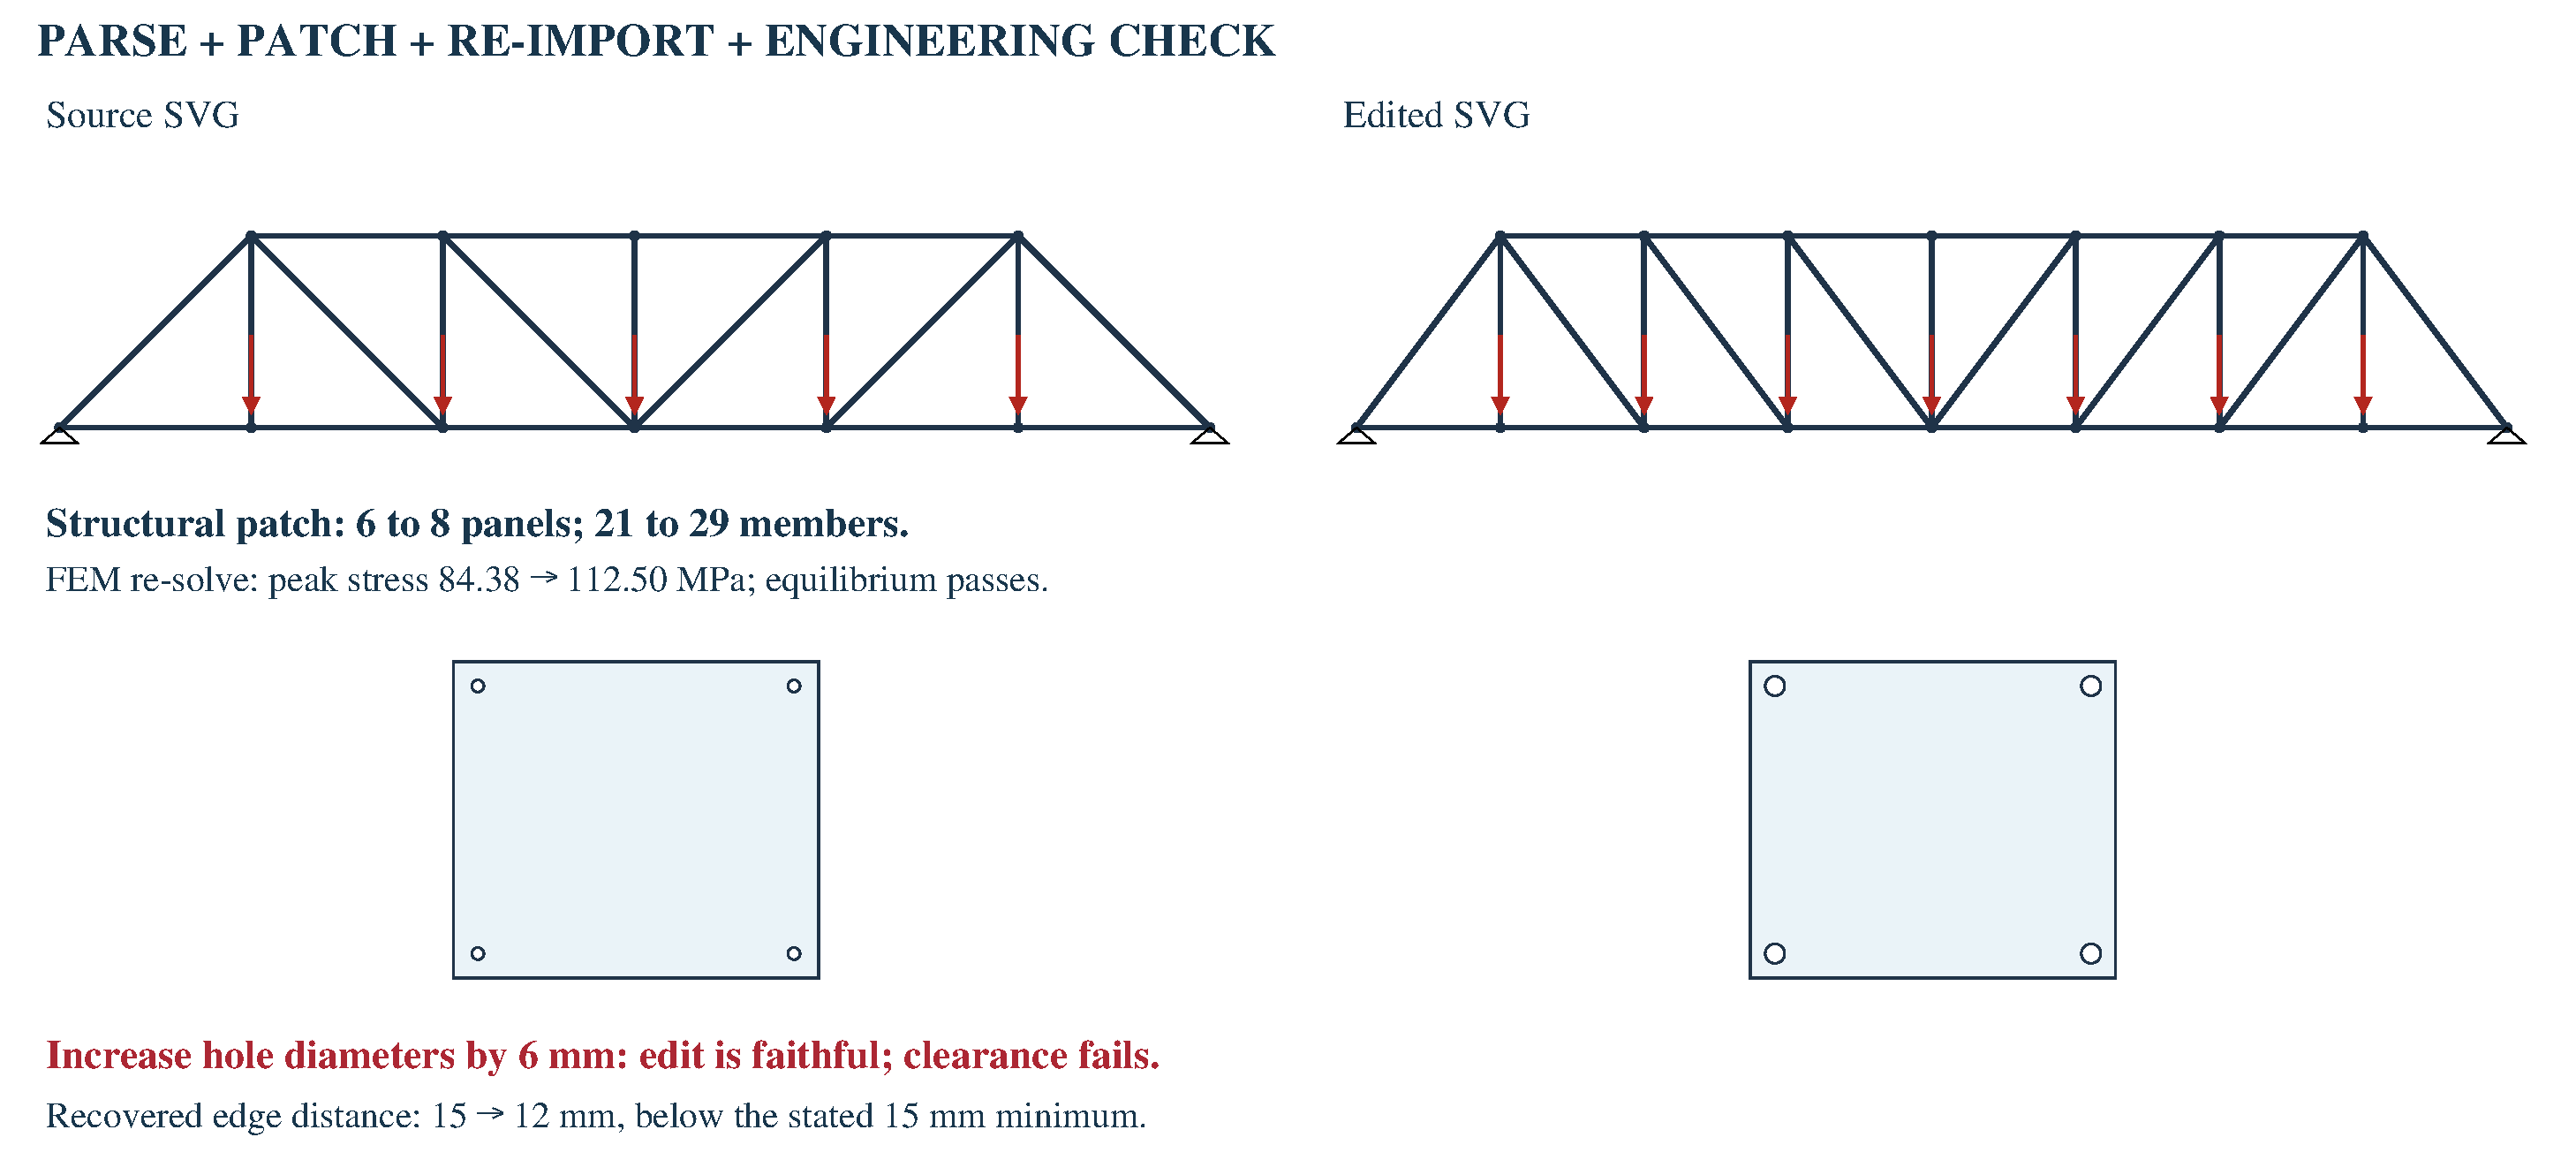
\includegraphics[width=\linewidth]{figures/editor-overview.pdf}
\captionsetup{hypcap=false}
\captionof{figure}{\textbf{Two edits, re-imported and re-checked.}
\textbf{Top:} ``Change the bridge to 8 panels'' on a Pratt truss with span $L{=}12$\,m, depth $h{=}2$\,m and
member area $A{=}800$\,mm$^2$ ($E{=}200$\,GPa). The 53-operation patch repositions 36 existing elements,
inserts 8 members, 4 joints and 2 load arrows, and updates the title, giving 29 members. The drawing specifies
$P{=}15$\,kN per loaded node, so the loaded bottom-chord nodes increase from 5 to 7 (total load 75\,$\to$\,105\,kN).
Axial FEM on the re-imported drawing gives a peak member stress of 84.4\,$\to$\,112.5\,MPa, equal to the midspan chord
force $PLn/(8h)$ divided by $A$ for $n{=}6\,{\to}\,8$ panels, and a peak displacement of 8.95\,$\to$\,11.85\,mm; the relative
equilibrium residual is below $10^{-13}$. This confirms that the edited truss is solvable and in equilibrium. No stress
limit is applied, so it does not show that the bridge is safe.
\textbf{Bottom:} ``Increase all hole diameters by 6\,mm'' on a 300$\times$260$\times$9\,mm plate whose hole centres lie
$c{=}20$\,mm from both adjacent edges. The two-operation patch changes $d$ from 10 to 16\,mm and updates the hole note,
matching the target SVG tree exactly. The clear edge distance $e{=}c-d/2$ falls from 15 to 12\,mm, below the 15\,mm minimum.
The source holes already sit at that minimum, so with fixed centres the rule allows only $d\le2(c-15)=10$\,mm;
16\,mm holes need $c\ge23$\,mm. The request is infeasible as stated: the editor applies it without moving the holes,
and the check reports the violation. This is a geometric clearance rule, not FEM. Geometry is cropped from the source
and edited SVGs, with labels omitted and colors normalized.}
\captionsetup{hypcap=true}
\label{fig:teaser}
\end{strip}

\begin{abstract}
We study engineering SVG editing through source-tree parsing, parsed and validated patches, and
physical or geometric checks on the recovered output. The evaluated implementations cover electrical and hydraulic networks, axial trusses
and perforated plates. A learned 1.5B network editor reaches 100\,\% on 1,000 held-out edits and
\editOneFiveHard\,\% on larger networks under identifier addressing, paired with circuit and hydraulic
solvers. Separately, a bounded deterministic truss/plate editor reproduces all 40,000 targets in a saved
pipeline audit and flags 699 faithful plate edits that violate clearance rules. Worked SVG examples
show member resizing, load changes, structural topology patches and hole enlargement. Axial FEM
recomputes stress, displacement and equilibrium; geometric checks measure edge distance and ligament.
Saved \astra cases expose a false pipe-network verdict and repeated refusal to analyse a correctly
edited 21-member frame. Results retain the input contract and checker of each evaluated editor.
\end{abstract}

\section{Introduction}
\label{sec:intro}

Editing an engineering drawing requires several linked updates. Moving a column changes member lengths;
changing a bridge's panel count changes connectivity and loading; enlarging holes changes clearances;
and modifying a pipe redistributes flow. A useful SVG editor must preserve the intended design, update
its geometry and annotations, and recompute the quantities affected by the edit.
\Cref{fig:teaser} shows two implemented examples: a bridge edit followed by FEM and a faithful plate
edit whose reduced edge distance is flagged by a geometric check.

Markup or pixel similarity alone cannot establish these properties. SVG-editing
benchmarks~\cite{svgeditbench,scidiagramedit} measure output similarity, while engineering-reasoning
benchmarks~\cite{feabench,fem_bench,pdeagent_bench} evaluate numerical answers or simulation tasks.
Our question concerns the delivered artifact: does the edited SVG describe the requested design,
and what happens when that design is analysed under the stated assumptions?

We use an edit--recover--check workflow. The editor parses the source into a scene tree, predicts or constructs a patch, parses and validates
that patch, and applies it to the original SVG. Structural operations insert nodes when topology changes. A family-specific importer
then recovers the produced drawing. The applicable solver or geometry checker evaluates that recovered
result. Edit fidelity and engineering acceptance are reported separately: a correct edit can introduce
a violation, and passing one check does not certify every aspect of a design.

The network implementation, \ours, recovers visible wire and pipe connectivity, component symbols and
labels without identifiers or hidden metadata. A learned patch editor supplies the edits; modified nodal
analysis and hydraulic flow--head equations supply the verdicts. The structural/mechanical extension
uses bounded edit interpretation and importers for trusses and plates, followed by axial FEM or
manufacturing-geometry checks. A separate frame harness uses a supplied physical model and checks
returned member geometry before a planar-frame FEM solve. We report these contracts explicitly rather
than pooling their scores into a single cross-domain accuracy.

\paragraph{Contributions.}
\begin{itemize}
\item \textbf{Editing followed by verification of the resulting SVG.} The supported routes cover
circuits, pipe networks, axial trusses and perforated plates. Worked examples expose the requested
revision, changed geometry and recomputed engineering quantities (\cref{sec:structures}).
\item \textbf{A learned network editor with a drawing-grounded verifier.} The 1.5B identifier-addressed
editor achieves 100\,\% on 1,000 held-out network edits and \editOneFiveHard\,\% on larger networks.
The verifier passes \numControls{} analytical controls and recovers \roundTripTotal{} generated drawings
exactly (\cref{sec:method,sec:experiments}).
\item \textbf{Reproducible datasets and checked edit examples.} We provide \netEdits{} network edits,
a \hardEdits{}-edit harder network tier, and a saved 40,000-edit deterministic truss/plate pipeline audit.
The latter identifies 699 requested plate edits that are faithful but violate clearance rules.
These are pipeline results, not learned-editor accuracy (\cref{sec:data,sec:structures}).
\item \textbf{Audited analysis failures and limitations.} The saved \astra pipe error, repeated frame
analysis refusal, opaque-identifier control and 100-case cross-domain learned-patcher pilot show where
editing, interpretation and checking must be evaluated independently.
\end{itemize}

\section{Related work}
\label{sec:related}

\paragraph{Vector graphics generation and editing.}
Learned SVG generators model paths and primitives directly~\cite{carlier2020deepsvg} or emit SVG code with a
language-model decoder~\cite{rodriguez2025starvector}. Instruction-based SVG editing is benchmarked by
comparing the edited result with a reference image or markup~\cite{svgeditbench}, and scientific-diagram work
learns edits from paper revisions~\cite{scidiagramedit} or targets structure-faithful
generation~\cite{sciforma}. These methods treat a drawing as an image or a document. We treat an engineering
drawing as a specification of a physical network and score it by what that network does.

\paragraph{CAD and engineering design.}
Generative CAD models produce parametric construction sequences~\cite{wu2021deepcad,khan2024text2cad}, and
agentic systems couple language models to simulators for mechanics~\cite{mechagents} and finite-element
analysis~\cite{all_fem,vfeagent}. Benchmarks such as FEABench~\cite{feabench}, FEM-Bench~\cite{fem_bench}
and PDEAgent-Bench~\cite{pdeagent_bench} evaluate the reasoning or code that sets up a simulation. Our
verifier instead reads a finished two-dimensional drawing and reconstructs the model it implies, so it can
audit the artefact a designer or a model actually delivers.

\paragraph{Network analysis.}
Modified nodal analysis~\cite{ho1975mna} is the standard formulation for linear circuits. Pipe networks are
classically solved by loop corrections~\cite{hardycross1936} or by the gradient method on flows and
heads~\cite{todini1988} that underlies EPANET~\cite{rossman2000epanet}; we use Churchill's friction
factor~\cite{churchill1977}, which is continuous from laminar through fully rough flow. None of this is new.
What is new is running these solvers on networks recovered from free-form drawings, and using them as the
metric for text-guided editing.

\section{Network editing and drawing-grounded verification}
\label{sec:method}

\begin{figure}[t]
\centering
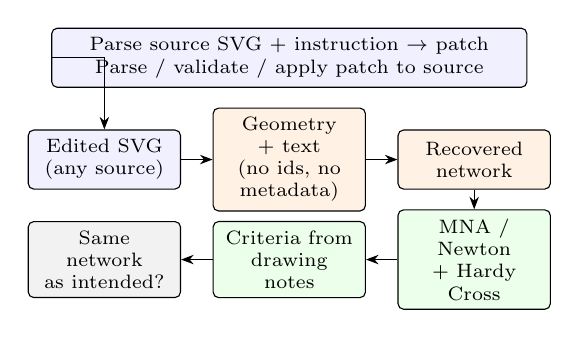
\begin{tikzpicture}[font=\scriptsize, node distance=2.5mm and 4mm,
  box/.style={draw, rounded corners=2pt, align=center, minimum height=7.5mm, text width=17mm, fill=#1},
  box/.default={white}, >={Stealth[length=1.6mm]}]
\node[box=blue!6] (svg) {Edited SVG\\(any source)};
\node[box=orange!10, right=of svg] (geo) {Geometry $+$ text\\(no ids, no metadata)};
\node[box=orange!10, right=of geo] (net) {Recovered\\network};
\node[box=green!8, below=of net] (solve) {MNA / Newton\\$+$ Hardy Cross};
\node[box=green!8, left=of solve] (check) {Criteria from\\drawing notes};
\node[box=gray!10, left=of check] (score) {Same network\\as intended?};
\draw[->] (svg) -- (geo);
\draw[->] (geo) -- (net);
\draw[->] (net) -- (solve);
\draw[->] (solve) -- (check);
\draw[->] (check) -- (score);
\node[box=blue!6, text width=58mm, above=2.5mm of geo] (editor) {Parse source SVG $+$ instruction $\to$ patch\\Parse / validate / apply patch to source};
\draw[->] (editor.west) -| (svg.north);
\end{tikzpicture}
\caption{\textbf{The network implementation of \ours.} An edited network drawing is read as built: geometry and labels become a network, the
network is solved, and the result is checked against the criteria printed on the drawing and compared with
the intended design. The network importer does not read identifiers or metadata.}
\label{fig:pipeline}
\end{figure}

\paragraph{Patch-based editing.} The editor receives the parsed source SVG and an instruction and emits
operations on that source tree. A patch parser checks the operation schema; policy validation checks
targets and allowed mutations before execution. The executor serializes the updated tree as the output
SVG. The engineering importer then reads this executed artifact for verification. The full-SVG outputs
in the saved Astra experiment are a separately identified baseline; they are not the editing interface
of the patch model.

\paragraph{Task.} A source drawing $S$ of a network and an instruction $u$ (\eg ``Add R7 = 10\,$\Omega$ in
parallel with R1'') define a target design $D^\star$. An editor returns a drawing $\hat S$. We ask two
questions of $\hat S$: does it describe $D^\star$ (\emph{edit correctness}), and does the network it describes
satisfy the criteria stated on the drawing (\emph{verdict})? Both are decided by recovering a network
$\mathcal{R}(\hat S)$ from the drawing and solving it.

\subsection{Recovering a network from a drawing}
Recovery parses the SVG with transforms applied and rejects scripts, external references, clipping and
masking. It then reads only what is visibly drawn.

\paragraph{Connectivity.} Stroked straight segments are candidate conductors (for pipe networks, only heavy
strokes). \Cref{fig:connectivity} shows the connection rules. A segment endpoint lying in the interior of
another segment is a T-junction and splits it; a filled
junction dot splits every segment passing through its centre. Two segments that merely cross stay
unconnected, which is the drafting convention for both schematics and piping plans. Endpoints closer than
$\tau = 10^{-3}$ drawing units are merged. For circuits, all points joined by wire form one electrical node.
For pipe networks, nodes are points of degree $\neq 2$, dotted points and points on a reservoir outline, and
every chain of segments between two nodes is one pipe. A $90^\circ$ turn along a chain is an elbow; other
bend angles are rejected.

\begin{figure}[t]
\centering
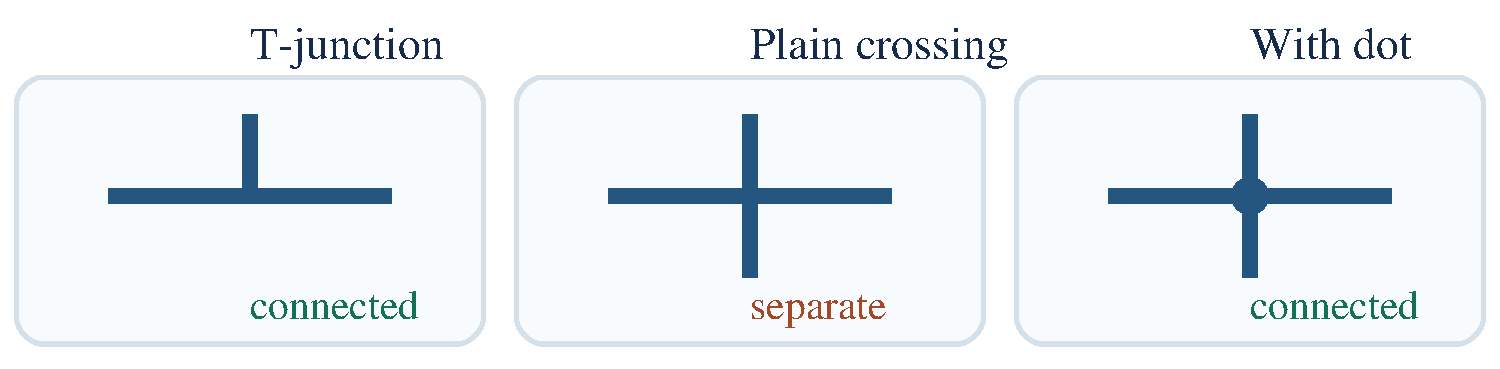
\includegraphics[width=\linewidth]{figures/connectivity-conventions.pdf}
\caption{\textbf{Connection conventions read from visible geometry.} A segment ending on another makes a
T-junction. Two segments that cross remain separate unless a filled dot marks their intersection. The same
rules apply to wires and pipes.}
\label{fig:connectivity}
\end{figure}

\paragraph{Components.} A rectangle whose two short-side midpoints coincide with conductor endpoints is a
resistor between the corresponding nodes. A circle is classified by where conductors meet it, not by its size:
if a conductor passes through its centre it is a junction dot, and if exactly two conductors end on its rim it
is a voltage source, whose positive terminal is the one nearer the ``$+$'' mark inside it. Filled rectangles
touched by pipe ends are reservoirs. Classifying by incidence rather than radius or stroke width keeps recovery
unchanged under uniform scaling of the drawing.

\paragraph{Values and criteria.} Labels are parsed with fixed grammars (\eg \code{R3 4.7 k$\Omega$},
\code{P5 320 m \O 150}, \code{J2 q=6 L/s z=10 m}) and assigned one-to-one to the nearest component or pipe,
within a reach proportional to the drawing's own scale (the median resistor body or pipe segment). Design
criteria are read from the drawing's notes: the resistor power rating and supply fuse; the pipe roughness,
elbow loss coefficient, minimum pressure head and maximum velocity. A drawing that leaves any component
unlabelled, or has two labels competing for one component, is reported as unreadable rather than guessed at.

\subsection{Solving the recovered network}
\paragraph{Circuits.} We use modified nodal analysis~\cite{ho1975mna} with one grounded node per connected
part of the network, so a floating fragment carries no current and does not make the system singular. A source
whose terminals share a node, or a loop made only of sources, makes the system singular; such a drawing is
reported as ill-posed. The outputs are every branch current, every resistor's dissipation and every source's
current; the criteria are $P_R \le P_\text{rated}$ for each resistor and $|I_V| \le I_\text{fuse}$ for each
source.

\paragraph{Pipe networks.} For pipe $p$ from node $a$ to node $b$ with flow $Q_p$, the head loss is
\begin{equation}
h_p(Q_p) = \Big(f(\mathrm{Re}_p,\varepsilon/D_p)\,\frac{L_p}{D_p} + n_p K_\text{elbow}\Big)
\frac{v_p |v_p|}{2g},
\end{equation}
where $v_p = 4Q_p/(\pi D_p^2)$, $f$ is Churchill's friction factor~\cite{churchill1977} and $n_p$ is the number
of elbows counted from the drawing. We solve jointly for pipe flows and junction heads,
\begin{equation}
h_p(Q_p) = H_a - H_b \;\;\forall p, \qquad
\textstyle\sum_{\text{in}} Q_p - \sum_{\text{out}} Q_p = q_j \;\;\forall j,
\end{equation}
with reservoir heads fixed, by Newton's method with backtracking~\cite{todini1988}, stopping at residuals below
$10^{-10}$\,m and $10^{-13}$\,m$^3$/s. Because Churchill's $f$ tends to $64/\mathrm{Re}$ in laminar flow, $h_p$
has a finite, non-zero slope at $Q_p = 0$ and the Jacobian stays regular when a flow reverses. As an independent
check, every network is also solved by Hardy Cross loop corrections~\cite{hardycross1936}, with multiple
reservoirs joined through a virtual datum node. The criteria are $|v_p| \le v_\text{max}$ for each pipe and
$H_j - z_j \ge p_\text{min}$ for each junction.

\subsection{Scoring an edited drawing}
An edit is \emph{correct} when $\mathcal{R}(\hat S)$ equals the target network $D^\star$ in two senses. The
first is topological: we compare, for every node, the multiset of named component terminals it touches, which
is a complete invariant of a network with named components, together with every component value and every
criterion. The second is physical: the two solutions agree, with currents within $10^{-9}$ relative plus
1\,pA, flows within $10^{-9}$\,m$^3$/s and heads within $10^{-7}$\,m. Markup is irrelevant: a drawing that
re-orders elements, renames identifiers or re-formats numbers is credited if it describes the same network,
and a drawing that is byte-for-byte plausible but disconnects a wire by $0.01$ units is not.

\subsection{Validating the verifier}
\label{sec:validation}
\Cref{tab:controls} lists the analytical controls. They include a balanced and an unbalanced Wheatstone
bridge; we initially chose bridge values that happened to balance, which made the ``unbalanced'' control
vacuous and hid a sign error, and we record this as a caution. Beyond the controls, \roundTripTotal{}
independently generated drawings (source designs and all their edits, over two seeds) recover to exactly
the network they were drawn from, as do all \datasetDrawings{} drawings in the released datasets.
Unit tests confirm four further properties: recovery is unchanged by stripping identifiers, shuffling
elements, translating and uniformly scaling the drawing by $\times0.25$ to $\times4$; a T-junction joins,
while a crossing joins only when dotted; moving only the ``$+$'' mark reverses every branch current; and moving
one wire endpoint by $0.01$ units breaks the connection. Two of these tests found real defects in the first
version. A fixed-radius rule for junction dots misclassified dots once the drawing was scaled up, and an
absolute current tolerance misjudged an edit whose two sources exactly cancel.

\begin{table}[t]
\centering
\footnotesize
\setlength{\tabcolsep}{3pt}
\begin{tabular}{@{}p{4.55cm}rr@{}}
\toprule
Control & \ours & Reference \\
\midrule
\controlRows
\bottomrule
\end{tabular}
\caption{\textbf{Analytical controls} for the two solvers. References are closed forms, an independent
bisection, or a second algorithm.}
\label{tab:controls}
\end{table}

\section{Network datasets}
\label{sec:data}

\paragraph{Resistor networks.} A design starts from a grid of $2$--$3 \times 3$--$5$ nodes. Edges are removed
at random while the graph stays connected and bridgeless (a bridge would carry no current), until $2$--$6$
independent cycles remain. Each edge becomes a resistor (E6 series, 10\,$\Omega$--6.8\,k$\Omega$), a plain wire
(20\,\%), or one of one or two DC sources (5--48\,V, random polarity). Designs are rejected if a resistor is
shorted, if sources form a loop, or if no current flows. Notes state a resistor power rating (0.25--2\,W) and a
supply fuse (0.1--1\,A). Drawings use standard symbols, with junction dots at nodes of degree three or more.

\paragraph{Water-distribution networks.} A random spanning tree of a $2$--$3 \times 3$--$5$ grid receives one to
three extra pipes to close loops. Some dead ends are pruned, and one or two reservoirs attach at the boundary.
Grid points of degree $\neq 2$, plus about a third of the rest, become junctions carrying a demand
(0--15\,L/s) and an elevation (0--30\,m). The remaining pass-through points become straight runs or
$90^\circ$ elbows. Pipes have lengths of 100--800\,m and nominal diameters of 80--300\,mm, and notes state the
roughness, elbow loss coefficient ($K=0.9$), minimum pressure head (10--20\,m) and maximum velocity
(1.5--2.5\,m/s).

\paragraph{Edits.} Each design receives four instructions. For circuits these are a resistor value change, a
source voltage change, a polarity reversal (two-source designs) or opening a branch (one-source designs,
provided the network stays solvable), and adding a resistor in parallel with an existing one, drawn as a
tapped branch. For pipe networks they are a diameter change, a demand change, removing a pipe (provided every
junction stays supplied and no reservoir is cut off), and adding a pipe between adjacent junctions (or, if
none exist, a length change). Target drawings are rendered from the edited design. The gold edit is a tree patch
derived between source and target SVG, applied with a validating executor and required to reproduce the
target exactly. A row is kept only if both drawings recover to their designs and, for pipes, Newton and Hardy
Cross agree to $10^{-9}$\,m$^3$/s.

\paragraph{Statistics.} \Cref{tab:data} summarises both tiers. The \emph{hard} tier uses $4$--$5 \times
5$--$6$ grids with $8$--$16$ independent loops for circuits and four to eight added pipes for water networks.
It is evaluation-only: no model is trained on networks of that size. Splits are by source design, so the four
edits of one drawing never cross splits.

\begin{table}[t]
\centering
\footnotesize
\setlength{\tabcolsep}{3.2pt}
\begin{tabular}{lrr}
\toprule
 & Main (v1) & Hard \\
\midrule
\dataRows
\bottomrule
\end{tabular}
\caption{\textbf{Datasets.} Loops are independent cycles of the recovered network (median, range). ``Verdict
flips'' are edits that turn a safe design unsafe or the reverse. All patches reproduce their targets and all
drawings recover to their designs.}
\label{tab:data}
\end{table}

\section{Learned network-editor evaluation}
\label{sec:experiments}

\paragraph{Astra failure probe.} We evaluate \astra (\code{gpt-6-astra}) through the Chat Completions API at medium
reasoning effort, with a 32{,}000-token completion cap, no tools, \code{store=false} and one sample per task.
\astra works in its natural mode: it receives the drafting conventions, the physical model (fluid properties,
friction law, loss conventions) and the criteria in the prompt, and it returns the complete edited SVG followed
by a JSON analysis stating the verdict, the violating components and the governing quantities. The edited SVG
is scored by \ours exactly as any other drawing (\cref{sec:method}), and the analysis is compared with the
solver's. Tasks are the first ten test edits by identifier for every (family, edit type) pair of the main tier
(100 tasks), and the first four of the hard tier (40 tasks). The API account ran out of credit during the run.
All \astraMainN{} main-tier and \astraHardN{} hard-tier tasks that completed are reported. Every circuit task
completed. The missing tasks are all pipe networks, which failed with ``no credits remaining'' (26) or a
dropped connection (12), and they are excluded rather than counted as failures.

\paragraph{Our editor.} \ours pairs the verifier with a small editor: Qwen2.5-Coder-Instruct~\cite{hui2024qwen25coder}
at 1.5B and 7B parameters, fine-tuned with LoRA~\cite{hu2022lora} (rank 16 on the attention projections) for two
epochs on the \netEdits{}-edit training split to map \emph{source SVG $+$ instruction} to a tree patch. The patch
is applied by a validating executor, and the resulting drawing is recovered and solved, so the verdict is
computed, not generated. Decoding is greedy. The hard tier is never seen in training. We compare two ways for
a patch to name the elements it changes. \emph{Positional} addressing uses the executor's native node
identifiers, where \code{n77} is the 77th element in document order. \emph{Id} addressing uses the element's own
SVG identifier (\code{\#R5-label}) and writes insertion at the end of a group as \code{"end"}. It is
translated to positional form before execution, so the two differ only in what the model must write.

\paragraph{Metrics.} \emph{Edit}: the edited drawing recovers to the target network. \emph{Verdict}: the stated
pass/fail matches the solver's. \emph{Violations}: the set of violating components matches exactly. \emph{All}: all
three at once. For systems whose verdict is computed by \ours, the verdict is taken from the solve of the edited
drawing, whether or not the edit was correct.

\begin{table*}[t]
\centering
\footnotesize
\setlength{\tabcolsep}{5pt}
\begin{tabular}{lcccc}
\toprule
System & Edit & Verdict & Violations & All \\
\midrule
\multicolumn{5}{l}{\textbf{Main tier} (same completed tasks for every system)} \\
\compareMainRows
\midrule
\multicolumn{5}{l}{\textbf{Hard tier} (8--16 loops for circuits; unseen in training)} \\
\compareHardRows
\bottomrule
\end{tabular}
\caption{\textbf{Edit and verdict accuracy}, \% (count), on the tasks \astra completed. ``\astra drawing $+$
\ours verdict'' keeps \astra's edited SVG but replaces its analysis with the solve of that drawing.}
\label{tab:compare}
\end{table*}

\subsection{Control cases and failure context}
\astra is an accurate editor of these drawings. Every one of its completed edits recovers to the target
network, including parallel branches drawn as tapped sub-circuits and pipes added between junctions, and it
never disconnected a wire or broke the drafting conventions. Its circuit analysis is exact on every
completed task, including hard-tier networks with up to 16 independent loops. We did not find the failure
boundary we expected for linear networks: at these sizes, unaided nodal analysis is within reach. Each answer
costs \$\astraMainCost{} on the main tier and \$\astraHardCost{} on the hard tier on average, and takes a median
of \astraMainSeconds{}\,s and \astraHardSeconds{}\,s respectively, with no truncated responses.

\subsection{Astra's silent wrong verdict}
\begin{figure}[t]
\centering
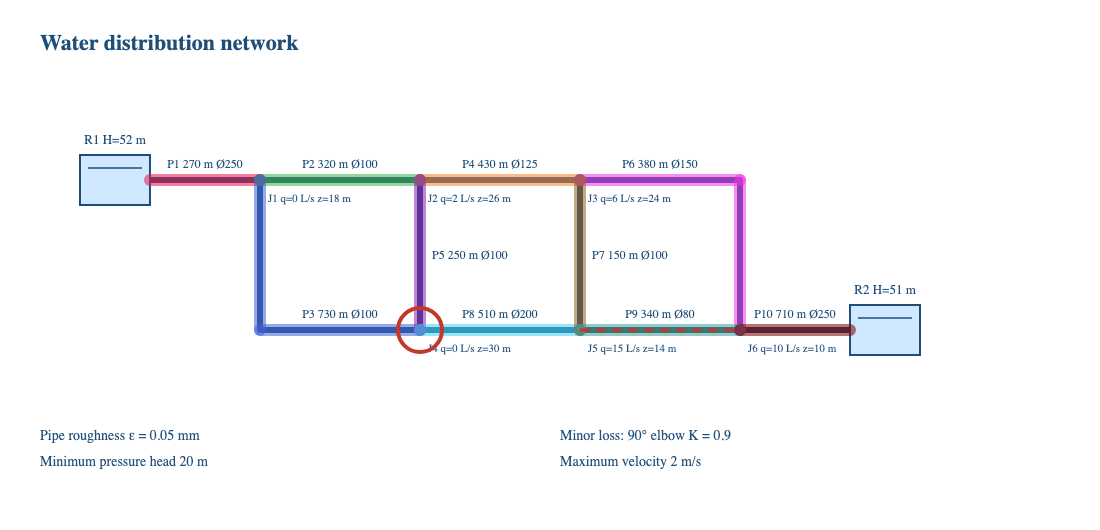
\includegraphics[width=\linewidth,trim=60 150 160 120,clip]{figures/astra-failure-pipe.png}
\caption{\textbf{Astra's wrong verdict on its edited SVG.} ``Change the length of P9 to 340\,m'' (dashed) in a two-reservoir
network with four loops. \astra's edit is correct, and it reports the minimum pressure head at J4 (circled) as
20.04\,m and the design as passing. Re-solving the drawing gives 19.23\,m, below the 20\,m minimum stated on
the drawing. Several of its pipe velocities are off by up to 67\,\%.}
\label{fig:failure}
\end{figure}

The only substantive error among \astra's completed network answers is in a nonlinear pipe network, and it is not flagged
(\cref{fig:failure}). The edit is right, but the analysis declares a failing design safe: it reports 20.04\,m
of pressure head where the drawing yields 19.23\,m against a 20\,m minimum, and its flows are wrong
throughout the loop that contains the edited pipe. Nothing in the answer
distinguishes it from the correct ones: it finished normally, used a similar reasoning budget, and presented
its numbers with the same precision. This is the failure mode a verifier exists for. It is rare (1 of
\astraMainN{} main-tier answers), it concentrates where the physics is nonlinear and the design sits near a
limit, and it cannot be detected from the answer itself. Replacing \astra's analysis with the solve of its
own drawing removes it (\cref{tab:compare}, second row). The source drawing already puts J4 below the 20\,m
limit (19.26\,m); the P9 edit leaves it below that limit (19.23\,m). \Cref{fig:astra-worked} shows both
drawings and the saved answer in detail.

\subsection{The small editor}
\begin{figure}[t]
\centering
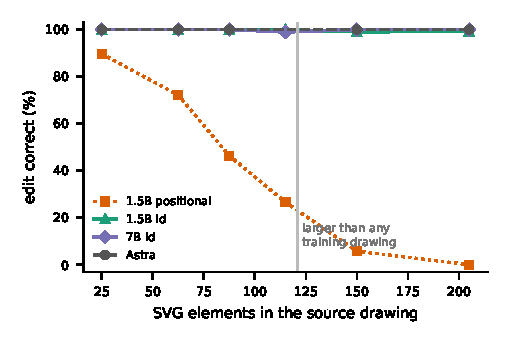
\includegraphics[width=\linewidth]{figures/size-curve.pdf}
\caption{\textbf{Edit accuracy against drawing size}, pooled over both tiers and binned by the number of SVG
elements in the source drawing (bins with at least five edits). The grey line marks the largest drawing in
the training split.}
\label{fig:size}
\end{figure}
\oursDiscussion

\begin{table}[t]
\centering
\scriptsize
\setlength{\tabcolsep}{1.8pt}
\begin{tabular}{@{}lccc@{}}
\toprule
Editor & Circuits & Pipes & All \\
\midrule
\oursFullRows
\bottomrule
\end{tabular}
\caption{\textbf{Our editor on the full test sets}: edit correctness by family and end-to-end accuracy (``pos.'' = positional, ``id'' = id addressing) on all 1{,}000 main-tier and \hardEdits{} hard-tier edits, \% (count).}
\label{tab:ours}
\end{table}

\subsection{Cost of a verified edit}
\costDiscussion

\section{Structural and mechanical SVG editing}
\label{sec:structures}

The engineering workflow extends beyond the network experiments through separate, bounded implementations.
\Cref{tab:domains} states which editor and checker are actually evaluated. This distinction matters:
the learned network model has not been evaluated as a general frame or truss editor.

\begin{table*}[t]
\centering\small
\setlength{\tabcolsep}{4pt}
\begin{tabular}{@{}p{2.1cm}p{3.4cm}p{4.3cm}p{5.7cm}@{}}
\toprule
Drawing family & Evaluated editor & Check on the output & Evidence and input contract \\
\midrule
Circuits / pipes & Learned 1.5B/7B tree patches & Circuit solve; hydraulic solve & 1,000 main and 400 hard edits; visible-geometry/label network importer \\
Axial trusses & Bounded deterministic edit & Axial FEM; equilibrium & 20,008 audited edits; visible geometry, sections, loads and supports in a fixed grammar \\
Perforated plates & Bounded deterministic patch & Hole/edge/ligament geometry & 19,992 audited edits; 699 faithful edits violate stated geometry rules \\
Planar frames & Saved \astra SVG edits & Geometry readback; frame FEM & Explicit physical model supplied; 21-member example, three analysis refusals in four attempts \\
Mechanical CAD & Saved \astra generation/edits & Task-specific shape checks & Ten completed hard-screen tasks pass; retained as controls \\
\bottomrule
\end{tabular}
\caption{\textbf{Implemented checks and evaluated editors.} Counts describe different protocols and are
not pooled. FEM and geometry checks apply only to their stated physical or manufacturing assumptions.}
\label{tab:domains}
\end{table*}

\subsection{Re-importing the edited structure}
The truss/plate route recovers an engineering representation from supported untagged SVG geometry and
visible annotations. A bounded request interpreter applies arithmetic and named parameter changes.
For fixed topology, the resulting target is converted to a tree patch, serialized, parsed, policy-checked
and applied to the original SVG. The actual patched SVG is imported again before verification.
Changing the panel count uses version-3 structural patches with subtree insertion and geometry replacement.
The bounded planner builds an internal target representation for patch derivation; the delivered SVG is
always obtained by applying the serialized, parsed and validated patch to the original source. The
21-to-29-member bridge example uses 53 operations: one text edit, 32 attribute edits, four geometry
replacements and 16 subtree insertions. Re-import and FEM check the executed result. This is a
deterministic patch compiler, not an evaluated learned topology-patch predictor.

\paragraph{A concrete parsed patch.} In the section-depth example, the source parser assigns the
section annotation the scene address \code{n34}. The serialized edit is:
\begin{lstlisting}
{"version":2,"operations":[
  {"op":"set_text","targets":["n34"],
   "text":"Section: 30 x 40 mm"}]}
\end{lstlisting}
The parser resolves this address against the source tree; the executor changes that annotation and
preserves the remaining elements. Re-importing the output recovers the larger axial area and FEM
reports peak stress 5.930\,MPa instead of 11.861\,MPa. Scene addresses belong to their parsed source;
they are not universal component identifiers.

\paragraph{Truss FEM.} For each pin-jointed member, the recovered endpoints determine its length $L$
and direction; visible section dimensions determine area $A$, and the material note supplies $E$.
The axial element stiffness is $EA/L$ times the direction-cosine matrix. Assembly and the recovered
support conditions give $K_{ff}u_f=f_f$. Member extension gives axial force and stress; support
reactions provide a global force and moment equilibrium check. The model assumes linear elasticity,
small displacement and nodal loading. The reported pass in this implementation is a numerical
equilibrium check, not a stress-allowable or buckling certification.

\paragraph{Plate geometry.} For circular holes in a rectangular plate, the importer recovers the
boundary, hole centres, diameters, thickness and stated clearance criteria. It checks boundary
crossing, hole overlap, edge distance and ligament, and reports net area and volume. For two holes,
the ligament is $\|c_i-c_j\|-r_i-r_j$; edge clearance is the distance from a centre to the nearest
boundary minus its radius. These are manufacturing-geometry checks; plate stress requires a separate
continuum model and is not inferred from the geometric pass.

\subsection{Verified SVG edit examples}
Five saved examples were replayed through the implementation for this revision; four reproduce the
earlier saved edited SVG trees, and the fifth is a clearance violation selected from the audited dataset.
\Cref{tab:worked-edits} lists their actual outputs. The source and edited SVGs, requests, applied patches
where applicable, and re-imported verification records are retained with the examples.

\begin{table*}[t]
\centering\small
\setlength{\tabcolsep}{4pt}
\begin{tabular}{@{}p{3.5cm}p{2.8cm}p{5cm}p{4.2cm}@{}}
\toprule
Request & Edit mechanism & Recomputed quantity & Check on delivered SVG \\
\midrule
Set all member depths to 40\,mm & Tree patch & Peak stress: 11.861 $\to$ 5.930\,MPa & Fidelity and FEM equilibrium pass \\
Double downward bridge load & Tree patch & Peak stress: 84.375 $\to$ 168.750\,MPa & Fidelity and FEM equilibrium pass \\
Change bridge to eight panels & Structural tree patch & 21 $\to$ 29 members; peak stress 112.500\,MPa & Connected output; FEM equilibrium passes \\
Enlarge six plate holes by 4\,mm & Tree patch & Edge: 25 $\to$ 23\,mm; ligament: 58 $\to$ 54\,mm & Stated clearance rules pass \\
Enlarge four plate holes by 6\,mm & Tree patch & Edge: 15 $\to$ 12\,mm & Faithful edit; 15\,mm edge rule fails \\
\bottomrule
\end{tabular}
\caption{\textbf{Replayed engineering edits.} These examples use the deterministic structural/mechanical
route. The bridge topology example keeps load per loaded node constant, so total load changes with
panel count. Stress is recomputed, but no material strength limit is tested by the truss equilibrium check.}
\label{tab:worked-edits}
\end{table*}

\paragraph{Full pipeline audit.} The saved dataset audit streams all 40,000 truss/plate SVG-edit rows
through edit interpretation, patch application, output re-import and the applicable checker. All 40,000
match the stored target tree and pass edit fidelity. All 20,008 truss edits satisfy FEM equilibrium.
Of 19,992 plate edits, 19,293 meet the geometric criteria and 699 violate edge-distance or ligament
requirements. The 699 are successfully executed edits whose consequences are flagged by the checker;
discarding them as editing errors would hide the distinction the workflow is designed to expose.
These synthetic, bounded requests demonstrate pipeline consistency rather than learned generalization.

\subsection{Learned editing across other drawing families}
A separate 7B patcher was trained on 8,000 lineage-disjoint synthetic examples and evaluated on 100
balanced held-out examples from five drawing families. It produces valid patches in 100/100 cases,
but exact target-tree equality in 59/100. The family counts are 4/20 building plans, 20/20 circuits,
6/20 furniture tables, 9/20 mechanical parts and 20/20 water piping. A drawing audit that allows
numeric serialization differences finds 60/100 outputs with both the intended recovered parameters
and internally consistent geometry. This is a different adapter, dataset and metric from the network
editor in \cref{tab:ours}. Mechanical dimension notes match in all 20 examples while 11 corresponding
drawings are geometrically inconsistent: checking annotations alone would overstate editing quality.

\paragraph{Frame and CAD analysis controls.} The saved 21-member frame example in
\cref{fig:astra-frame} passes geometry and dimension scoring in all four completed attempts; three
explicitly decline the requested analysis, while one calculates within tolerance. Its separate FEM
harness gives $u_x=3.5119$\,mm, $u_y=-0.1882$\,mm and peak stress $17.6837$\,MPa after the edit.
Ten hard-screen mechanical CAD outputs pass their geometric checkers, and six catalog-section
structural designs pass SVG readback and their FEM constraints. These positive controls and the frame
refusals establish checked examples under specific protocols; they do not establish a general CAD
solver or an Astra failure on every engineering family.

\section{Limitations and conclusion}
\label{sec:conclusion}

\paragraph{Limits of the evidence.} The drawing families are procedural and use bounded symbol and
annotation grammars. The learned network editor, deterministic truss/plate editor, separate frame
harness and cross-domain 7B patcher have different training and input contracts. Their results cannot
be pooled or transferred across domains. The network importer rejects unsupported symbols and label
placements. The structural importer covers idealised pin-jointed trusses; its FEM equilibrium pass
checks numerical consistency, not buckling, fatigue, joints or material strength. Plate clearance
checks supply no continuum stress analysis. The frame diagnostic receives an explicit physical model
and is outside the network importer's validated input domain.

The network Astra study uses one effort setting and one sample per task, with incomplete pipe coverage
because API credits ran out. Its single wrong verdict establishes a failure mode rather than a rate.
The repeated frame refusal concerns one edited structure, with one correct answer among four attempts.
The network editor's performance also depends on addressing: the saved 7B opaque-identifier control
falls from 398/400 to 154/400 correct hard edits. The broader learned patcher obtains 60/100 consistent,
intended drawings, so robust editing across arbitrary engineering sheets remains open. Numerical
velocity scoring for Astra uses a 0.01\,m/s absolute floor to avoid treating three-decimal rounding
near zero as a substantive error; edit and verdict scores are unaffected.

\paragraph{Conclusion.} The implemented workflow edits engineering SVGs and checks the design recovered
from the result. Its strongest learned result is accurate editing of the supported circuit and pipe
networks. Its structural/mechanical route demonstrates section and load edits, connected bridge
topology patching, and detection of clearance violations in correctly patched plates. FEM, circuit,
hydraulic and geometric checks make the consequences explicit. The resulting evidence identifies
both successful edits and the engineering criteria that a requested revision fails, with each claim
tied to the applicable model and delivered drawing.


{
    \small
    \bibliographystyle{ieeenat_fullname}
    \bibliography{refs}
}

\clearpage
\appendix
\section{Supplementary material}
\subsection{Prompt given to \astra}
System message:
\begin{lstlisting}
You are an engineering drafting and analysis assistant. Use your own reasoning; no external tools are provided. Do not claim you ran a solver.
\end{lstlisting}
User message for a circuit task, verbatim up to the source SVG, which follows in full:
\begin{lstlisting}
Instruction: Set R3 to 150 (*@$\Omega$@*).

Drawing conventions: straight lines are ideal wires. A wire that ends on another wire (a T) is connected to it; a filled dot also marks a connection; wires that cross without a dot are NOT connected. Rectangles are resistors and circles are ideal DC voltage sources; the '+' inside a source marks its positive terminal. Labels give component names and values.
Criteria (from the drawing notes): every resistor's dissipated power must not exceed the stated rating, and the magnitude of every source's current must not exceed the stated supply fuse rating.

Tasks:
1. Apply the instruction to the drawing, changing nothing else, and return the complete edited SVG.
2. Analyse the EDITED design and report whether it meets every criterion.

Answer with exactly two fenced blocks and nothing else: first ```svg containing the full edited SVG, then ```json containing {"verdict": "pass" or "fail", "violations": [names of every resistor or source that violates a criterion], "source_currents_A": {"V1": current delivered out of its + terminal, ...}, "max_resistor_power_W": {"name": "R?", "value": watts}}

Source SVG:
[complete source SVG]
\end{lstlisting}
For pipe networks the conventions paragraph and the JSON schema are replaced by:
\begin{lstlisting}
Drawing conventions: heavy lines are pipes; filled dots are junctions. A pipe runs between junctions or reservoirs and may turn through 90-degree elbows; each elbow adds the minor-loss coefficient K given in the notes. 'P# L m (*@\O{}@*)D' gives a pipe's length (m) and internal diameter (mm); 'J# q=.. L/s z=.. m' gives the demand withdrawn at a junction and its elevation; 'R# H=.. m' is a reservoir's fixed total head.
Analysis model: steady incompressible water, density 998 kg/m3, dynamic viscosity 1.002e-3 Pa s, g = 9.80665 m/s2; Darcy-Weisbach head loss with the Churchill (1977) friction factor and the pipe roughness in the notes; tee and junction losses neglected; pressure head at a junction = hydraulic head minus elevation.
Criteria (from the drawing notes): every pipe velocity must not exceed the maximum velocity, and every junction pressure head must be at least the minimum pressure head.

JSON schema: {"verdict": "pass" or "fail", "violations": [names of every pipe or junction that violates a criterion], "pipe_velocities_m_s": {"P1": speed, ...}, "min_pressure_head_m": {"name": "J?", "value": metres}}
\end{lstlisting}

\subsection{Worked \astra failure on the returned drawing}
\Cref{fig:astra-worked} shows the actual source SVG and \astra's returned SVG for the one completed network
answer with a substantive wrong verdict. The edit changes only P9's length from 290 to 340\,m; the returned
drawing equals the target SVG exactly. The source is already below its 20\,m pressure minimum at J4
(19.26\,m), and re-solving the edited SVG gives 19.23\,m. \astra instead reports 20.04\,m and \code{pass}.
Its reported velocity for P4 is 0.031\,m/s versus 0.095\,m/s from the edited drawing. These are analysis
errors on a correctly edited artifact. The orange and red marks in the figure are presentation overlays
added after the SVG was scored; they are not input to the verifier.

\begin{figure*}[t]
\centering
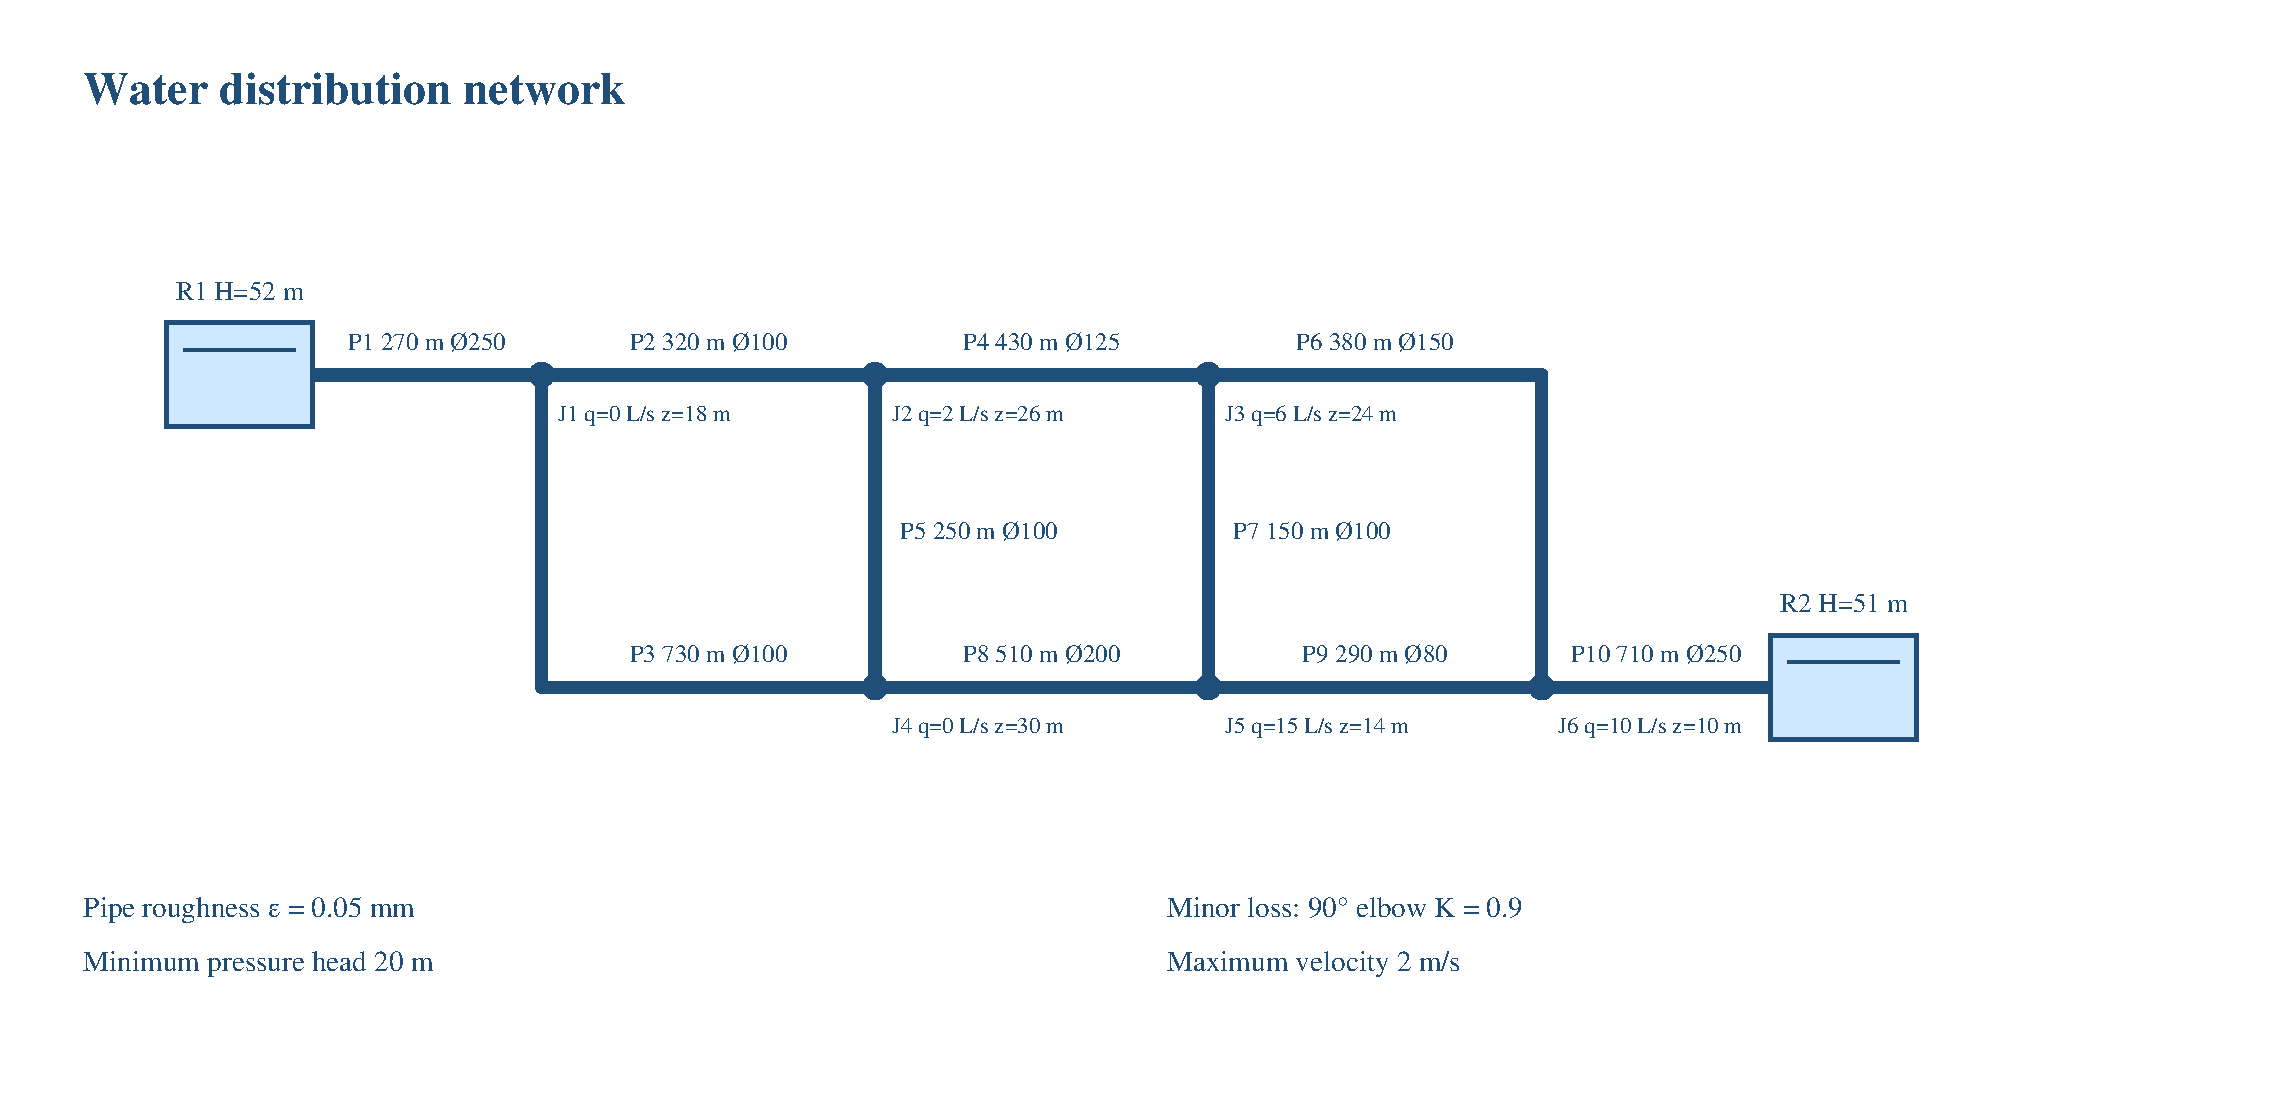
\includegraphics[width=.92\textwidth]{figures/astra-failure-source.pdf}\\[-2pt]
{\footnotesize (a) Source drawing: P9 is 290\,m; J4 is already below its pressure limit.}\\[3pt]
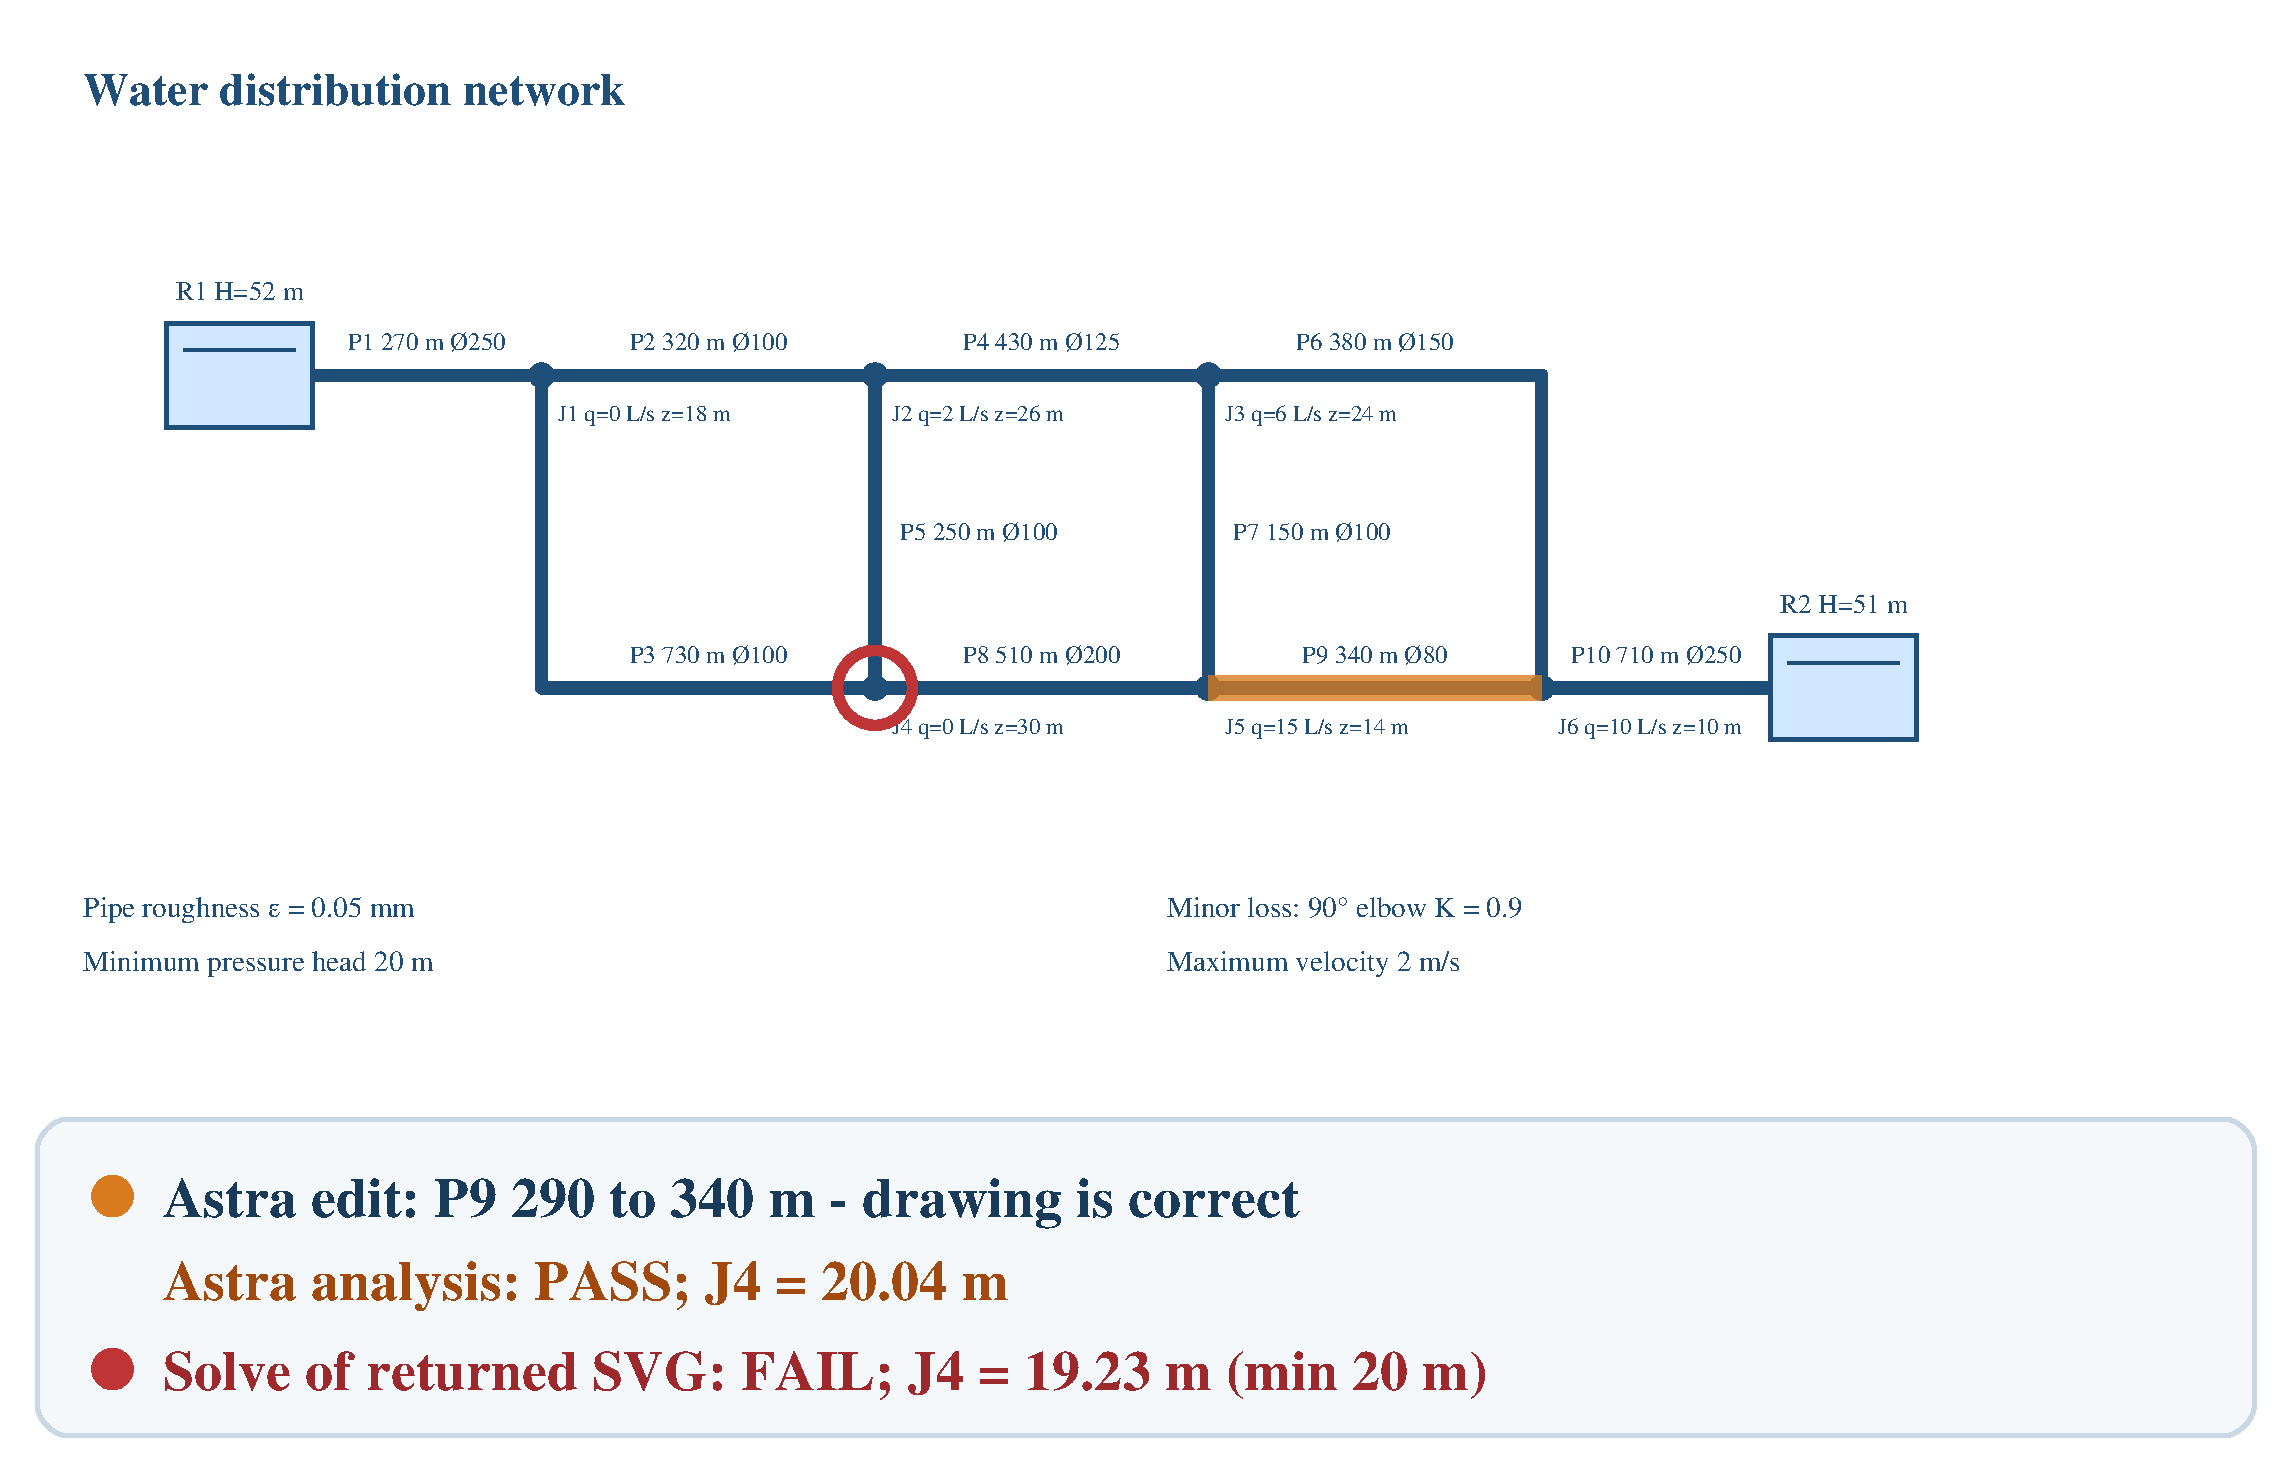
\includegraphics[width=.92\textwidth]{figures/astra-failure-response-annotated.pdf}\\[-2pt]
{\footnotesize (b) \astra's correct SVG edit (orange P9) with the missed J4 violation (red).}
\caption{\textbf{Astra failure, shown on the complete engineering drawings.} The two-reservoir, four-loop
network is edited correctly, but \astra's numerical answer declares it safe. The lower annotation contrasts
that answer with an independent solve of the returned SVG. Original unannotated SVGs were used for scoring.}
\label{fig:astra-worked}
\end{figure*}

\subsection{Separate structural-frame diagnostic}
To test whether the focus on circuits and pipe networks hid other engineering-drawing difficulties, we
re-audited saved \astra responses from a separate planar-frame study. The edit in
\cref{fig:astra-frame} moves one column grid from 3300 to 4000\,mm and increases the downward load at
the top-right joint from 53 to 68\,kN. The 21-member, three-storey frame has 27 degrees of static
indeterminacy. Its prompt supplied the explicit physical graph as well as the source SVG, and no
external solver. In three of four completed attempts on this same edit, \astra returned a drawing
whose member geometry and dimensions pass the independent scorer, but explicitly marked displacement
and stress as unavailable. In the fourth it gave values within 2\,\% of the frame FEM reference.
Re-solving each returned drawing gives $u_x=3.5119$\,mm, $u_y=-0.1882$\,mm and peak stress
$17.6837$\,MPa. This is a repeated refusal to calculate, not a wrong numerical safety claim.
It uses a separate planar-frame FEM harness; \ours does not verify these frames. Ten completed
mechanical CAD hard-screen tasks and six functional frame-sizing controls also passed their
respective saved-output audits, so neither provides an additional confirmed shape failure.

\begin{figure*}[t]
\centering
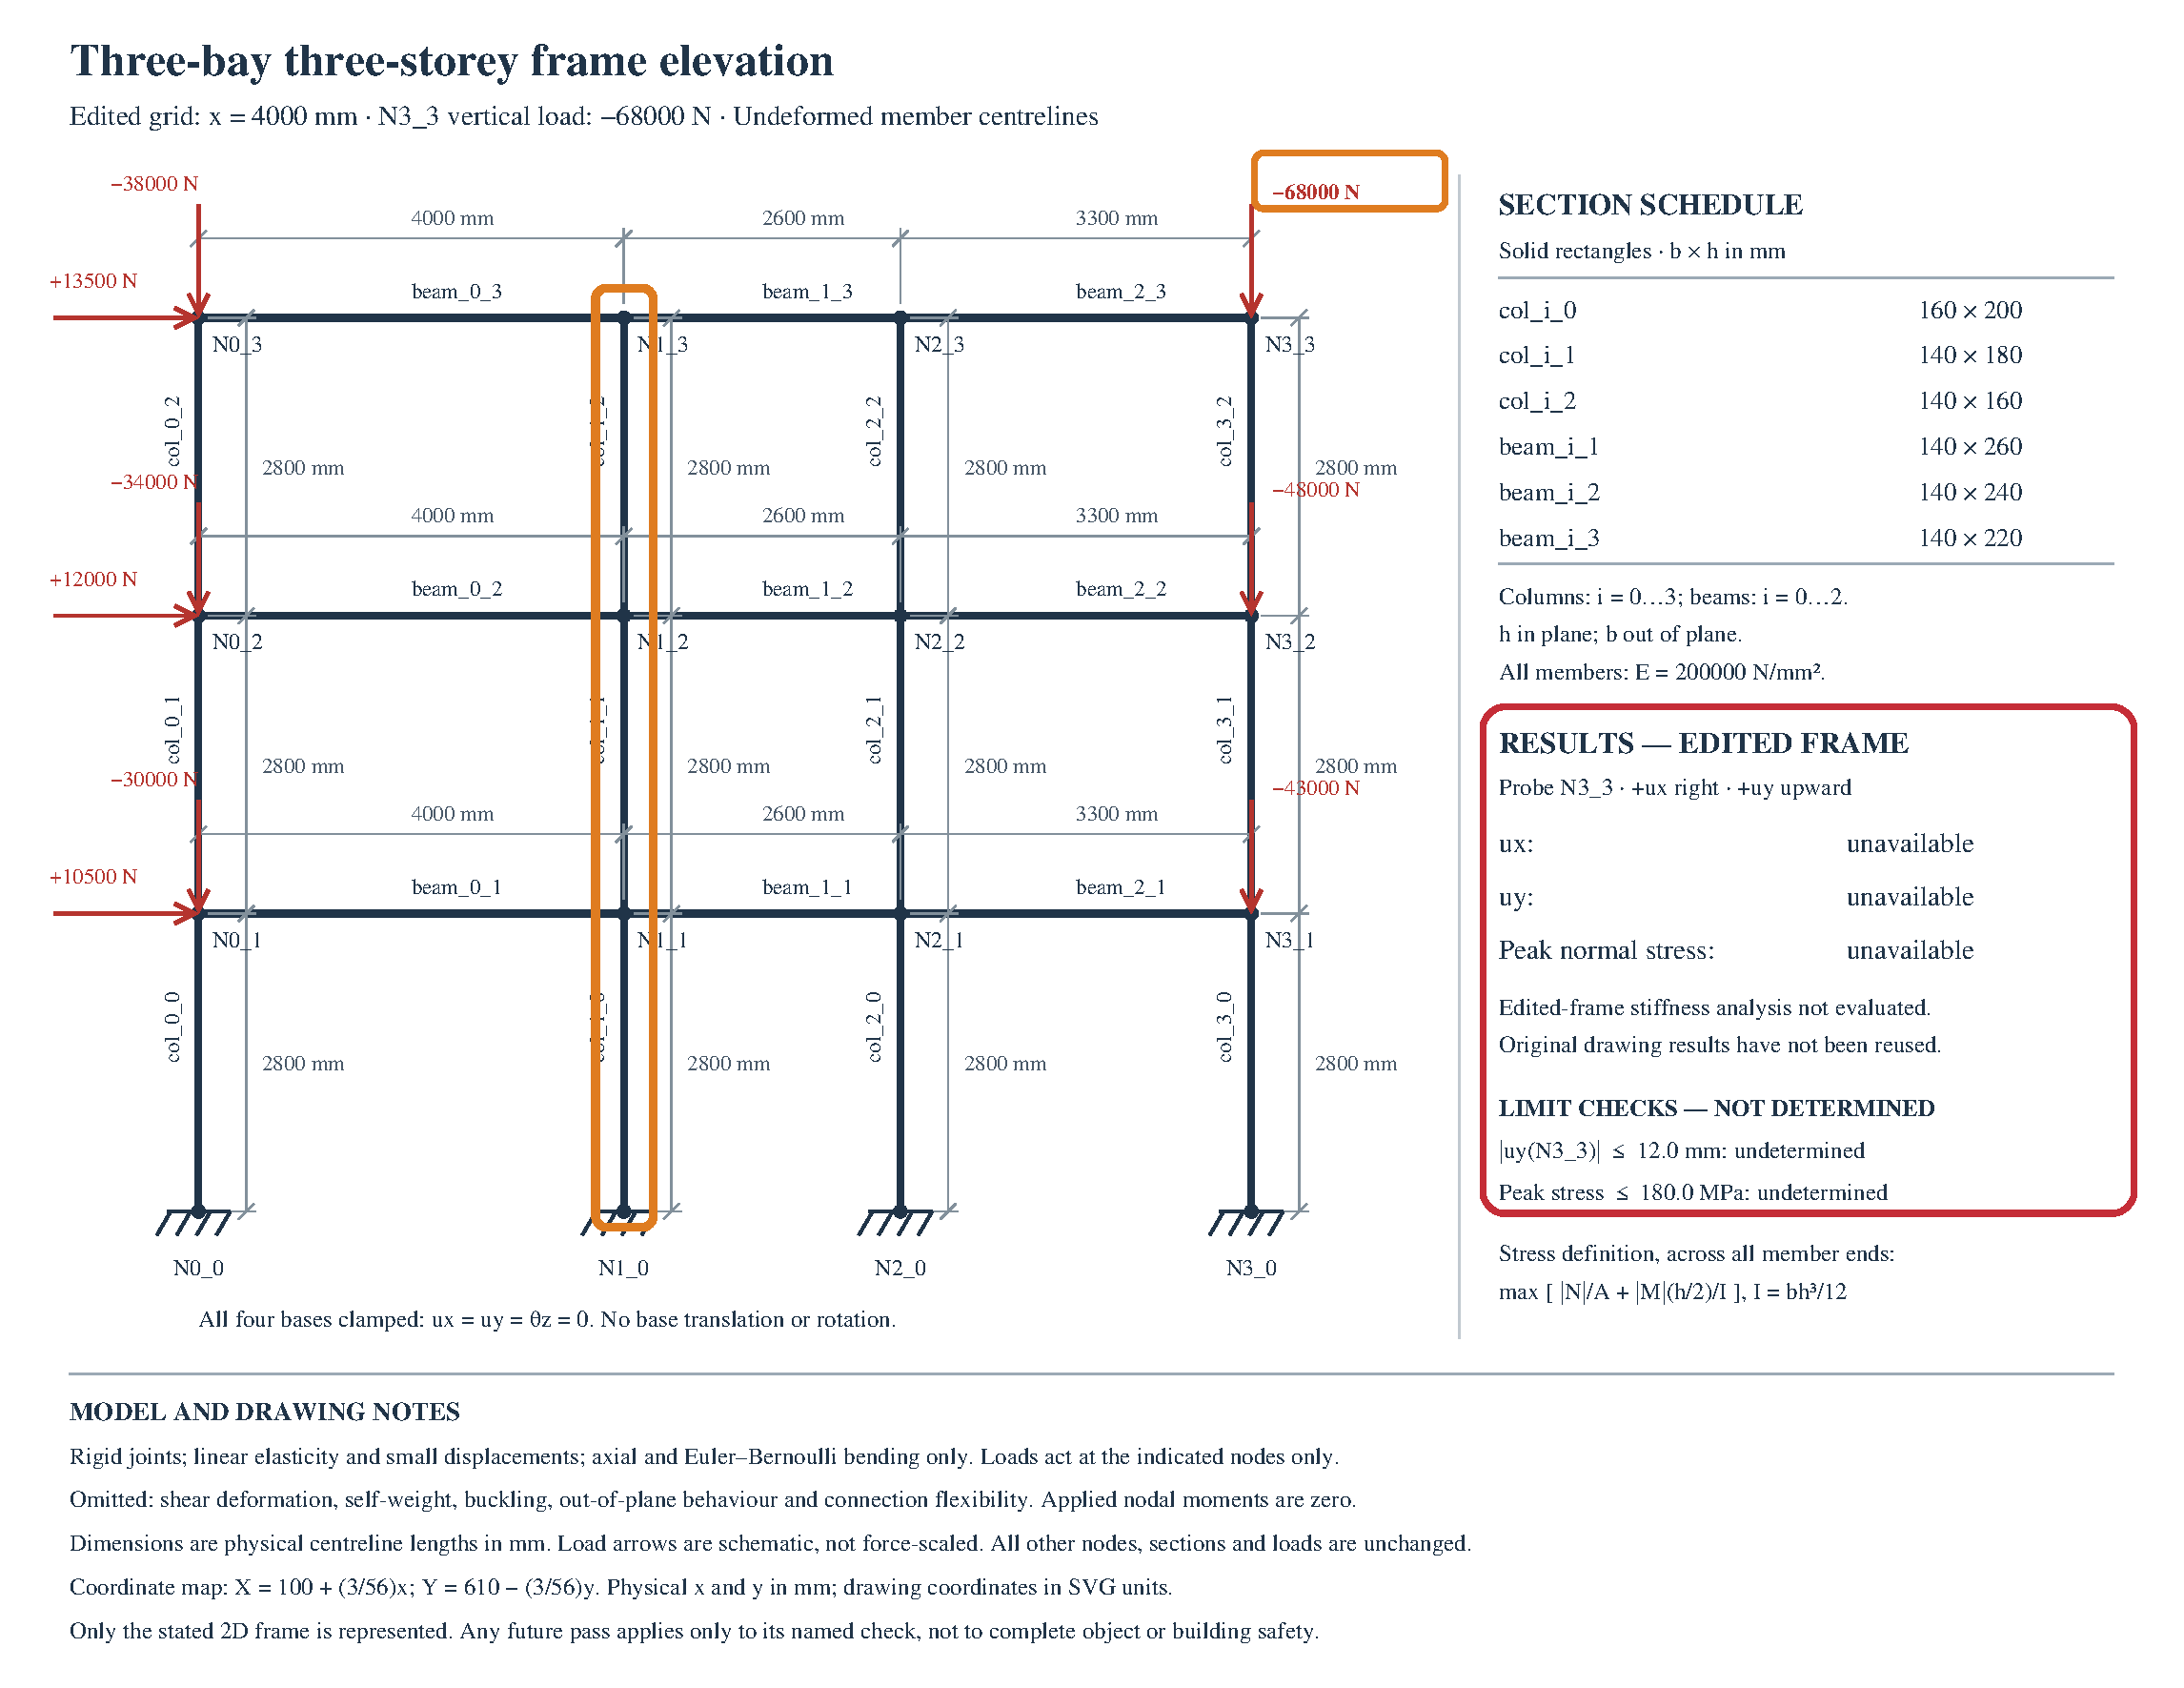
\includegraphics[width=.92\textwidth]{figures/astra-frame-decline-annotated.pdf}
\caption{\textbf{Astra's returned SVG for a 21-member frame edit.} The moved column grid and the
increased load are highlighted in orange; the red box encloses the unavailable analysis.
The editing is correct, but the requested stress and displacement analysis is absent in this
attempt and two of three other completed attempts. The fourth attempt calculates correctly.
Highlights are presentation overlays; the unmarked returned SVG was scored. This separate
structural diagnostic is not included in \ours's circuit and pipe-network benchmark.}
\label{fig:astra-frame}
\end{figure*}

\subsection{Results by edit type}
\Cref{tab:kinds} breaks end-to-end accuracy down by edit type. The one type on which \astra is below 100\,\%
is the pipe-length change that produced its silent wrong verdict (\cref{fig:failure}). Positional addressing
fails mostly on circuit edits, and id addressing is correct on every main-tier type at both model sizes.
\begin{table*}[t]
\centering
\footnotesize
\setlength{\tabcolsep}{5pt}
\begin{tabular}{@{}lcccc@{}}
\toprule
Edit type & \astra & 1.5B pos. & 1.5B id & 7B id \\
\midrule
\kindRows
\bottomrule
\end{tabular}
\caption{End-to-end accuracy (edit, verdict and violations all correct), \% (count). \astra on its completed main-tier tasks; \ours editors (positional or id addressing) on the full 1{,}000-edit main test set.}
\label{tab:kinds}
\end{table*}

\subsection{Training stability}
The first 7B training run, on an H100 NVL, diverged: the loss rose from 0.65 at step 20 to $3.0{\times}10^{4}$
at step 30 with a non-finite gradient norm, and the resulting adapter emits only ``\texttt{!}'' characters. Two
controlled 50-step reruns isolate PyTorch's cuDNN scaled dot-product-attention kernel: with it, the
gradient again became non-finite at step 30; without it, all steps were finite and the loss fell from
0.55 to 0.026. The reported 7B editor was retrained with that kernel disabled. The 1.5B editors,
trained on an RTX PRO 6000, never used it. The diverged run is retained, marked void and excluded
from every table. The trainer now stops at the first non-finite loss or gradient.

\clearpage
\onecolumn
\subsection{Worked structural and plate editing outputs}
\Cref{fig:structural-output} retains the visible engineering annotations of the replayed bridge and
six-hole plate examples. The bridge uses a parsed structural-tree patch; the plate uses a tree patch.
Both results are re-imported after editing. The exact source/output SVGs and verification JSON are
saved in the accompanying example run, so each numerical statement can be checked against the
produced artifact. The truss equilibrium pass is not a general structural safety certificate.

\begin{figure}[ht]
\centering
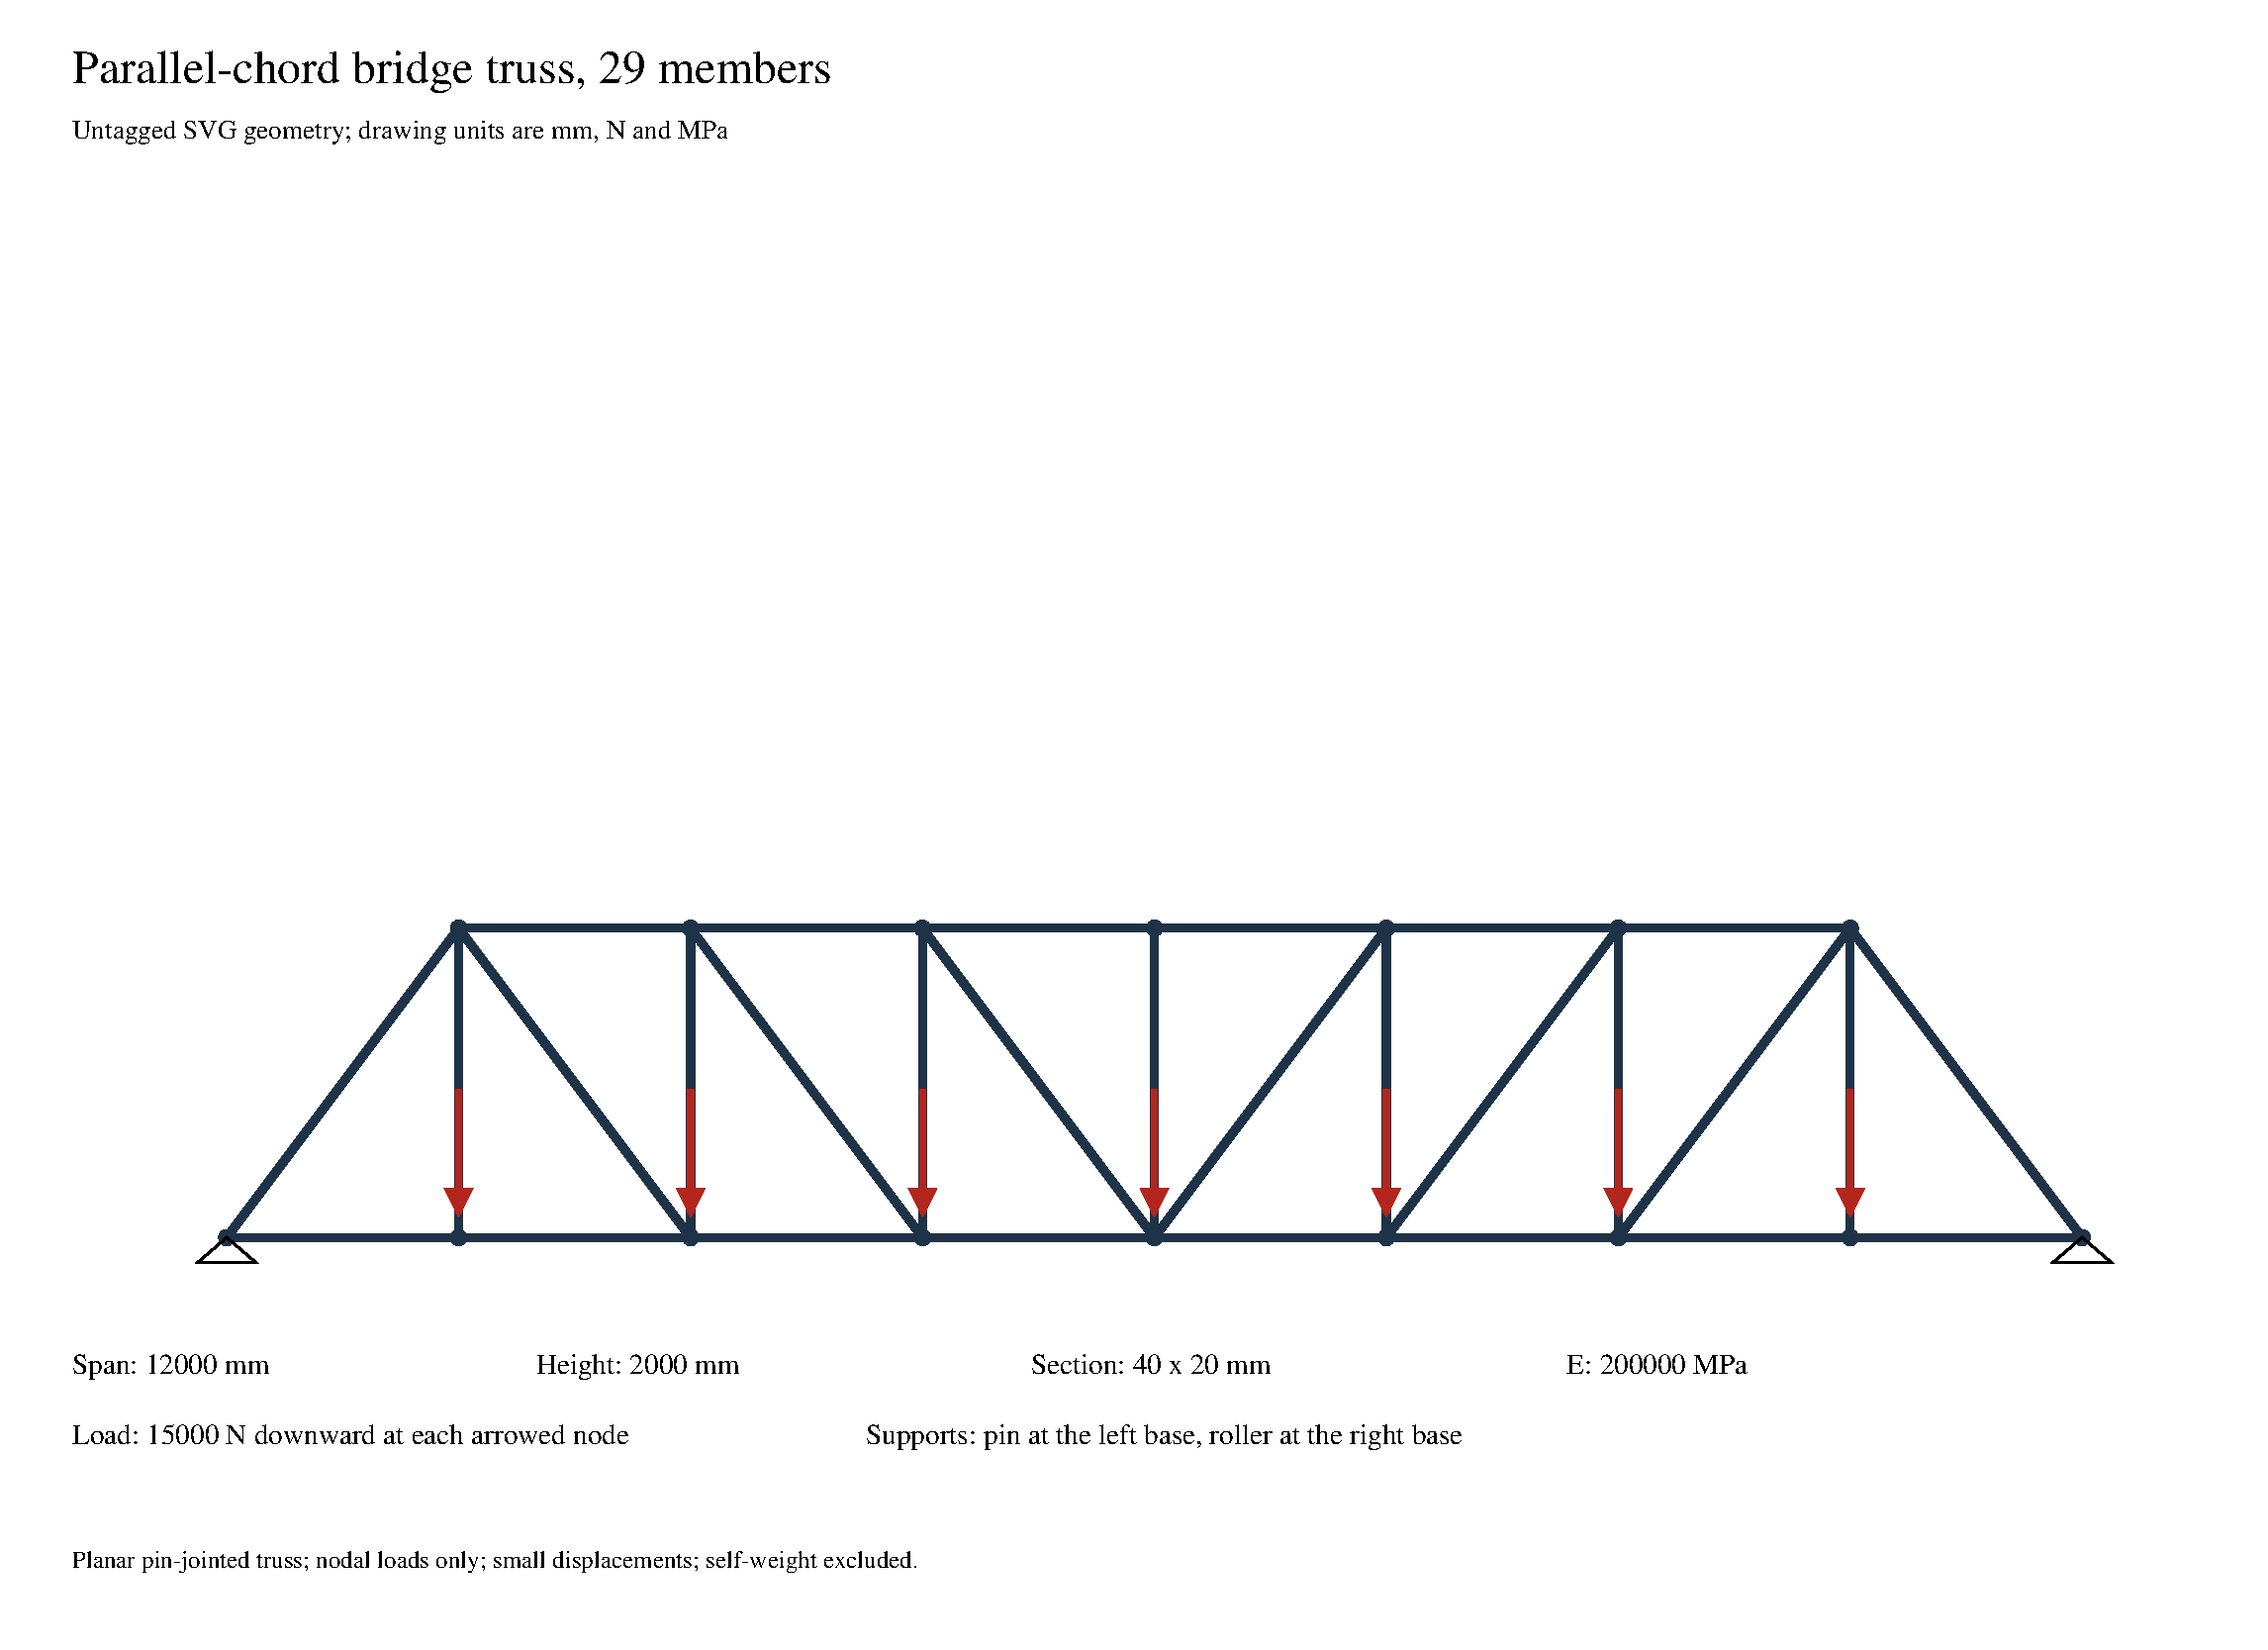
\includegraphics[width=.93\textwidth,trim=15 25 15 390,clip]{figures/editor-bridge-topology-edited.pdf}\\[3pt]
{\footnotesize (a) Delivered 29-member bridge SVG; FEM: peak stress 112.50\,MPa, maximum displacement 11.848\,mm.}\\[8pt]
\begin{minipage}{.48\textwidth}\centering
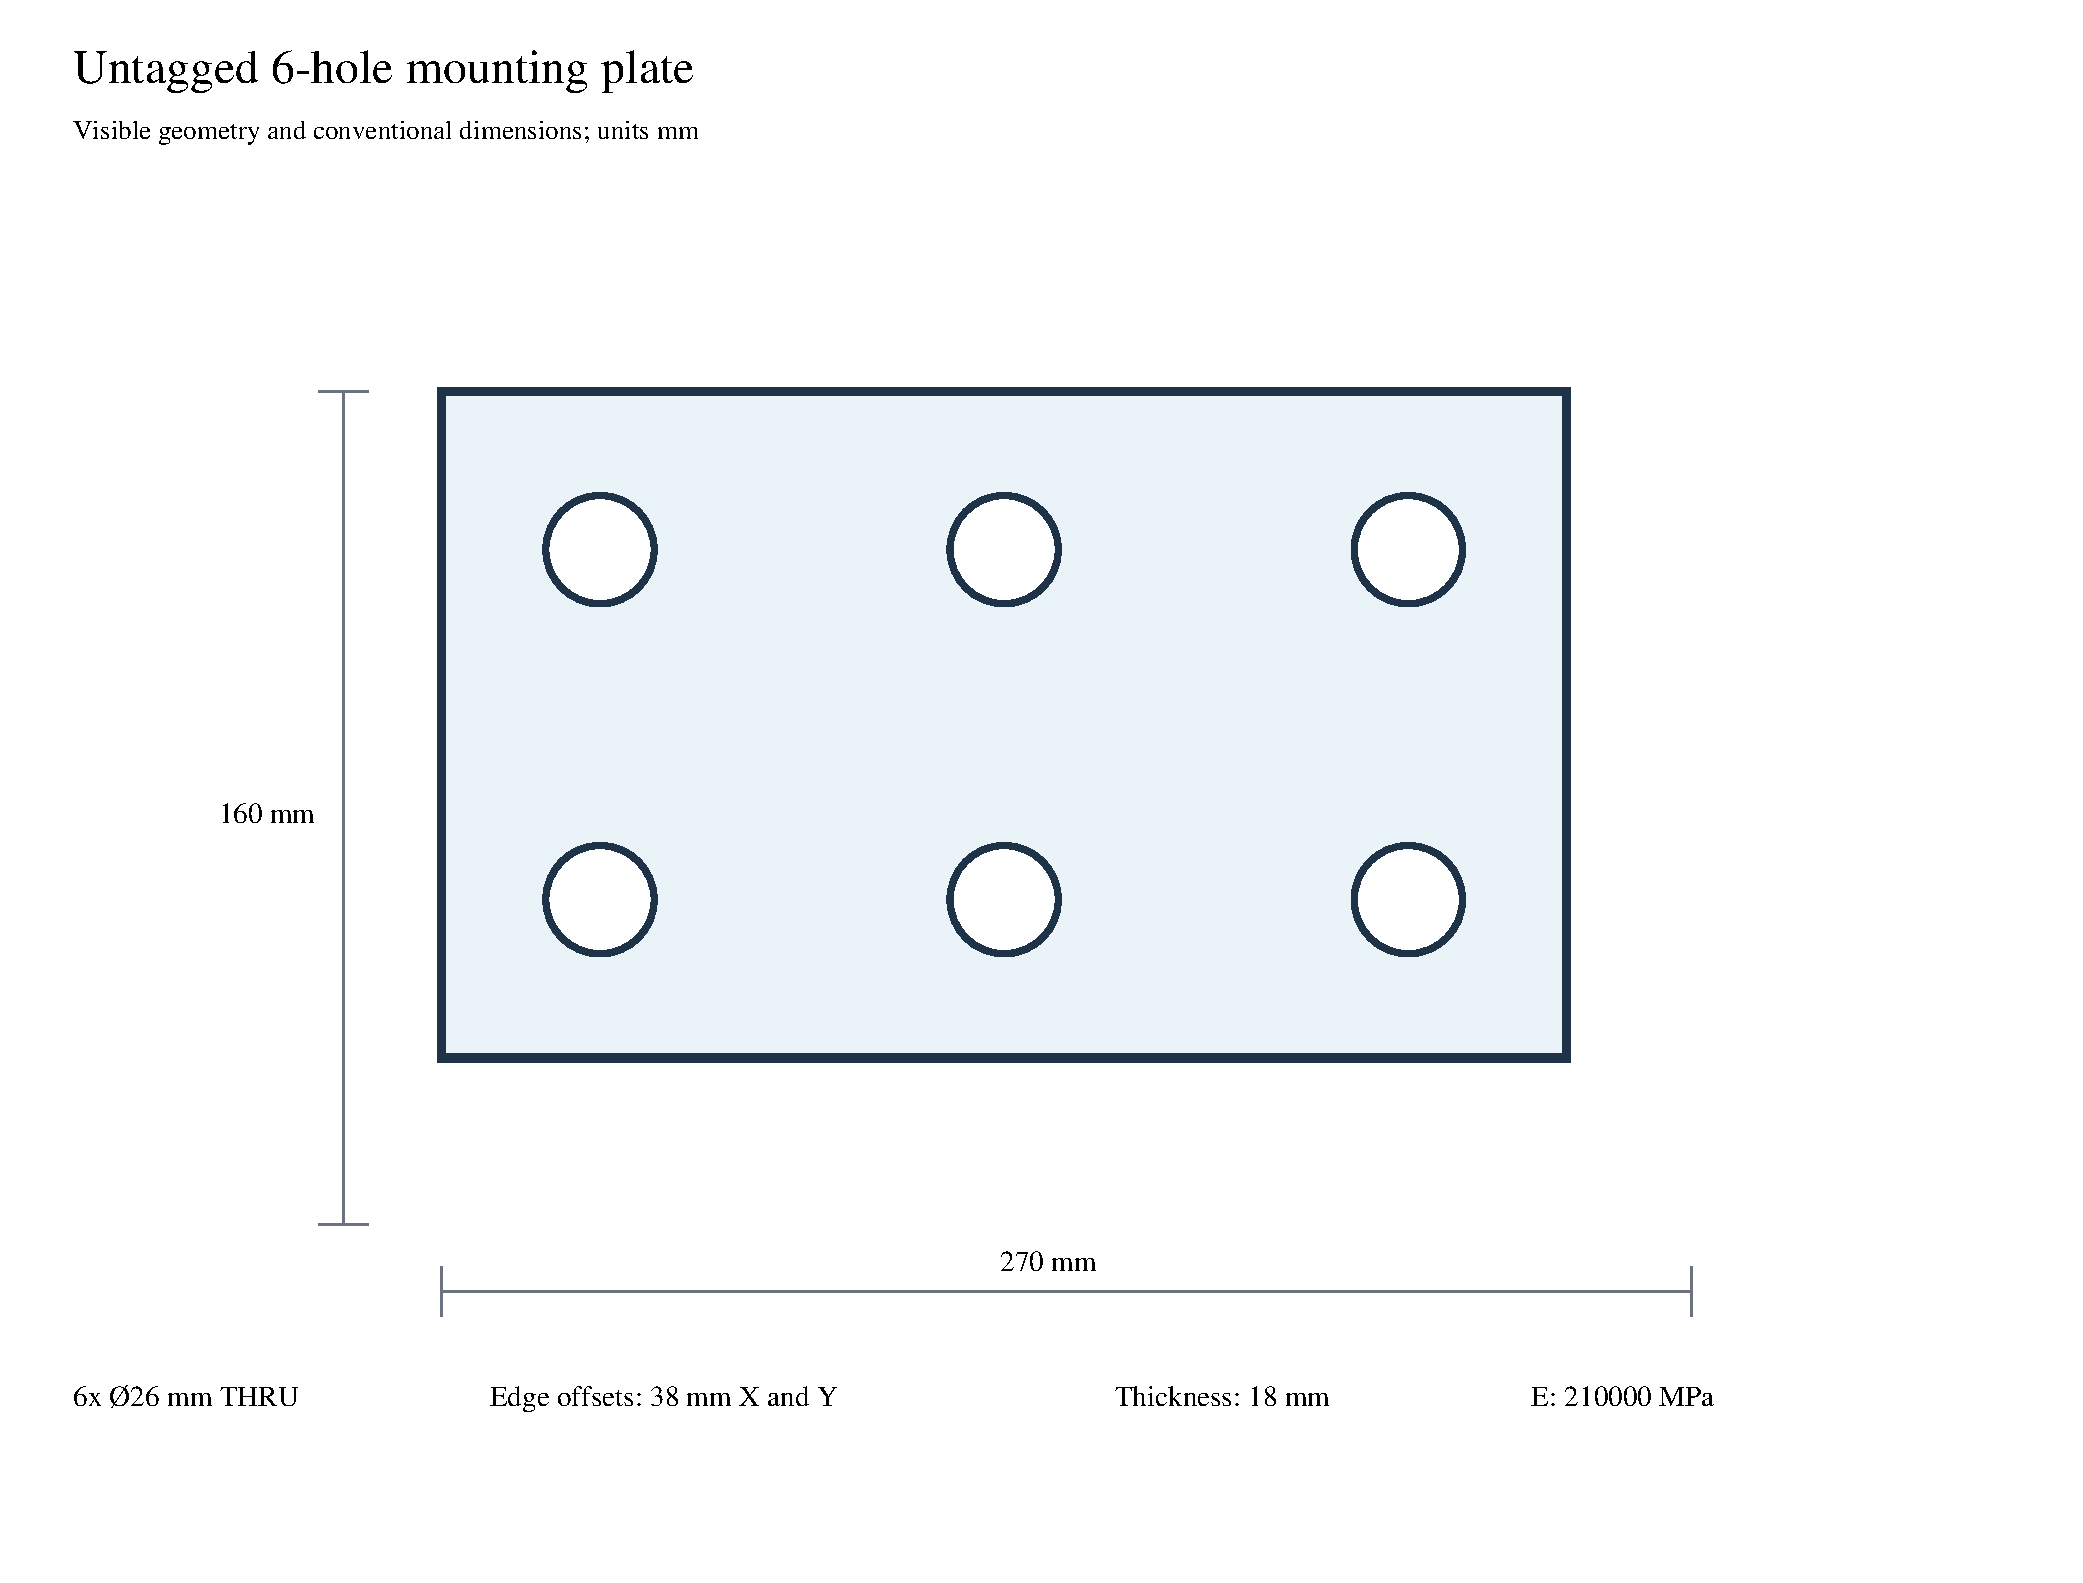
\includegraphics[width=\linewidth]{figures/editor-plate-holes-source.pdf}\\[-2pt]
{\footnotesize (b) Source six-hole plate.}
\end{minipage}\hfill
\begin{minipage}{.48\textwidth}\centering
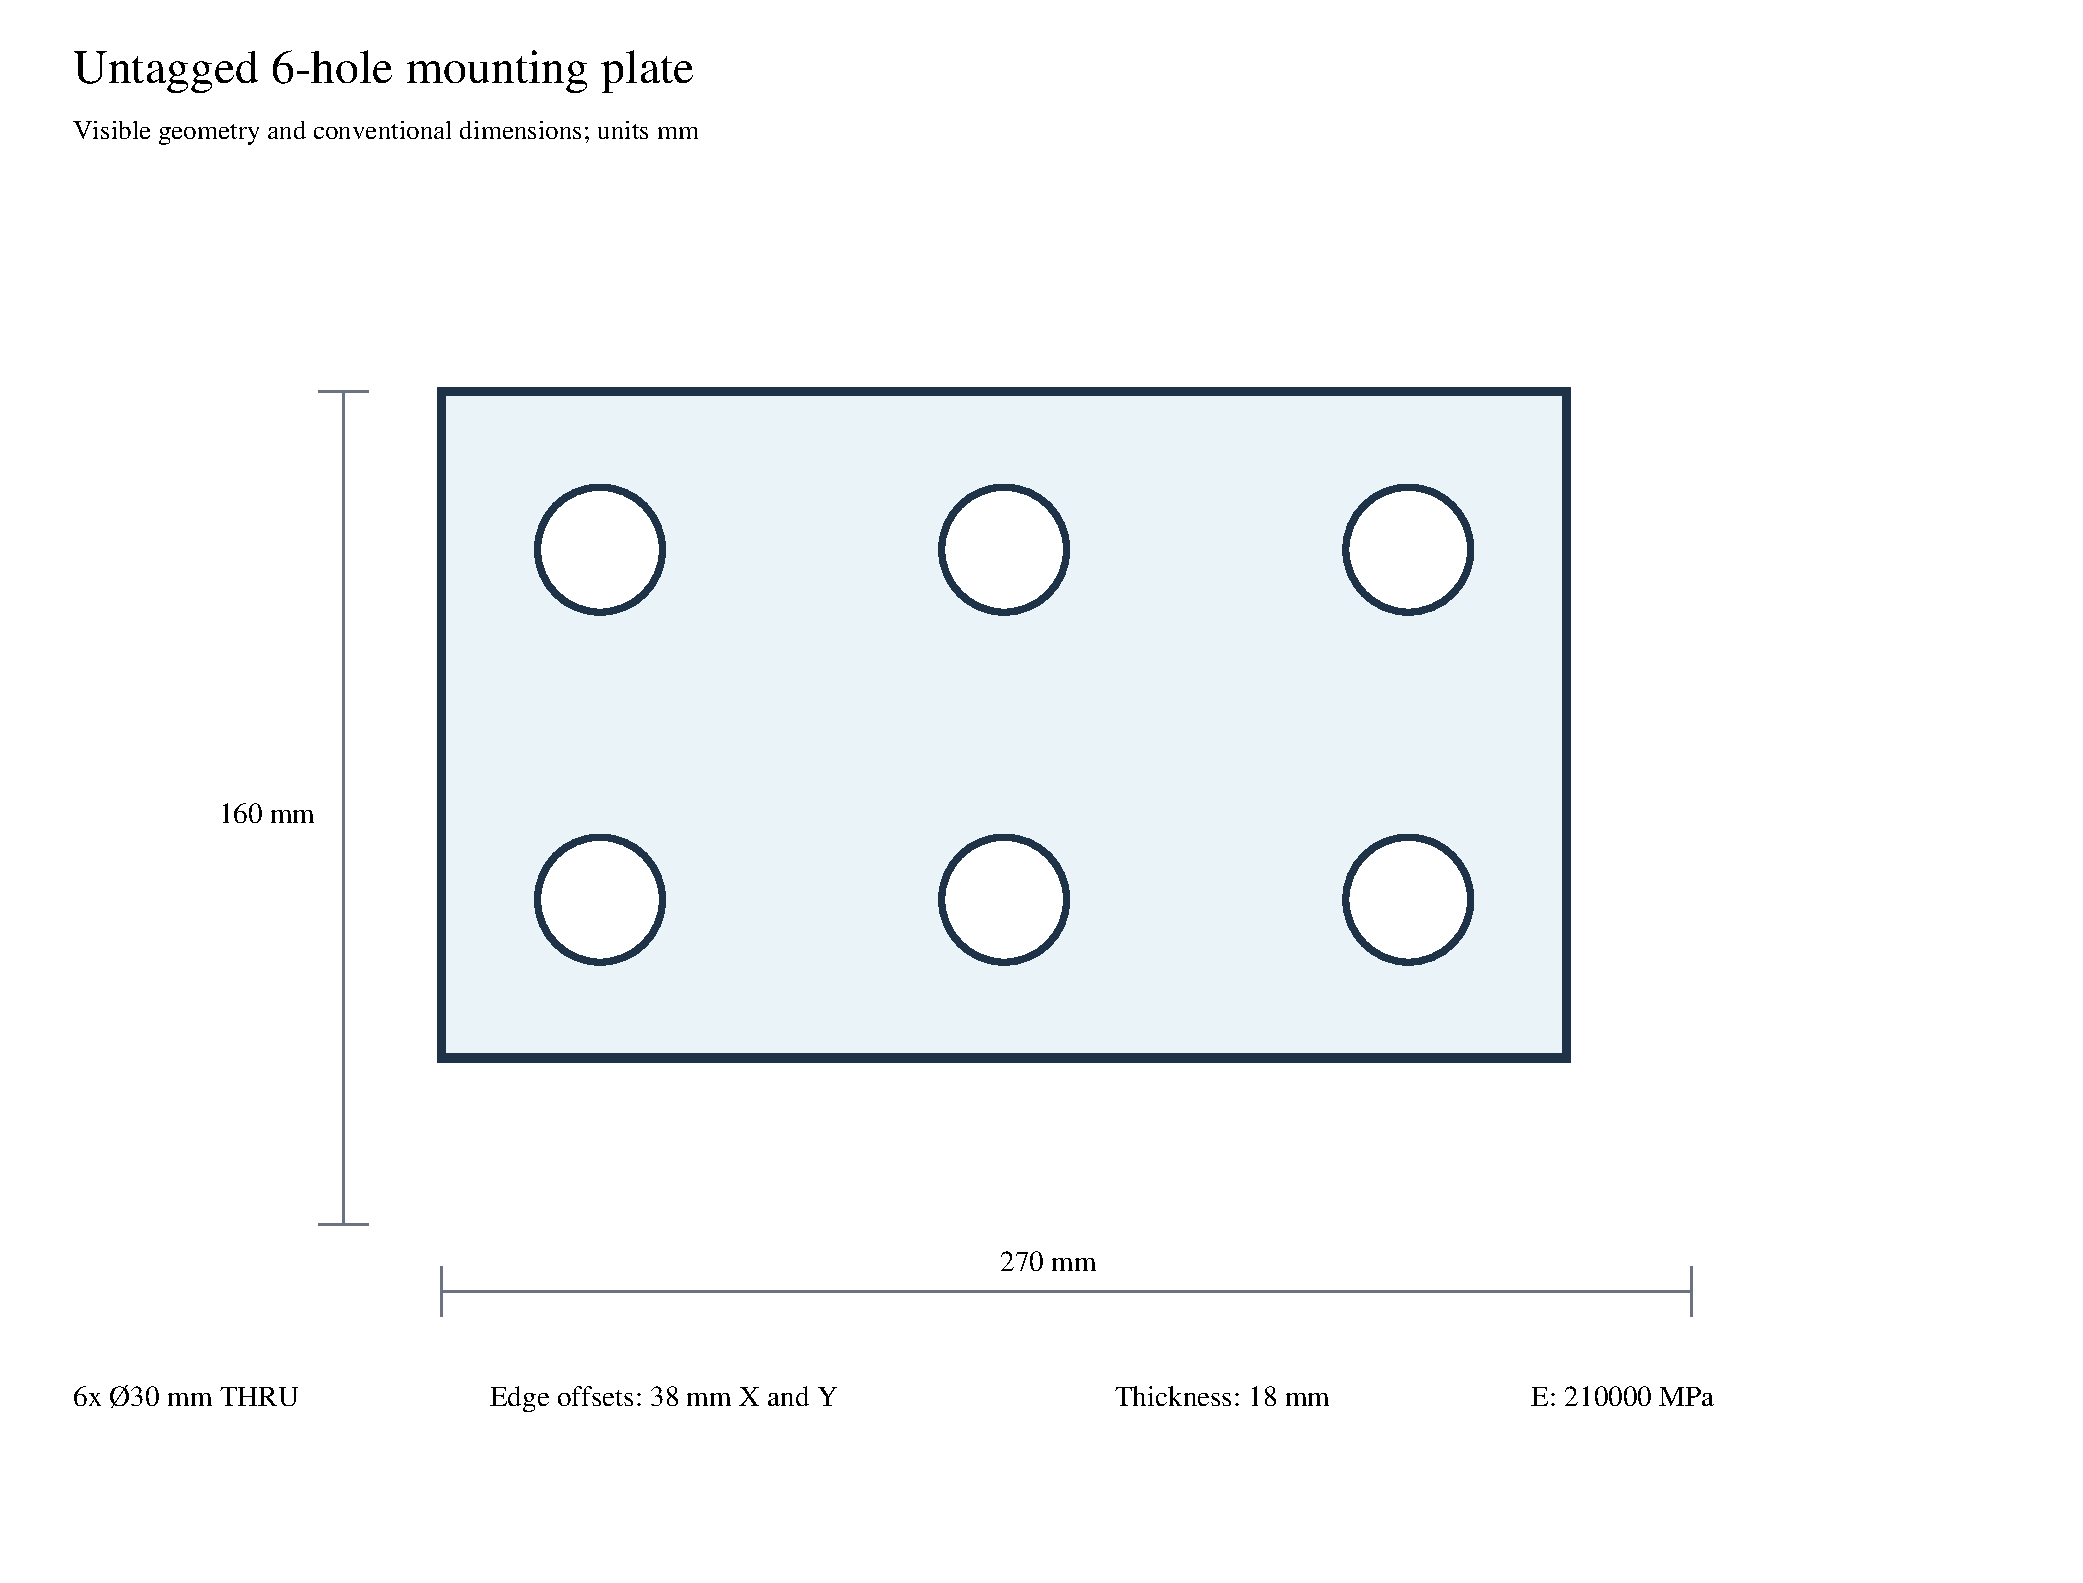
\includegraphics[width=\linewidth]{figures/editor-plate-holes-edited.pdf}\\[-2pt]
{\footnotesize (c) Hole diameters increased by 4\,mm.}
\end{minipage}
\caption{\textbf{Actual SVG outputs of the verified editor.} The bridge output preserves the stated
span, height, section and per-node loading while changing connectivity. The plate's recovered edge
distance changes from 25 to 23\,mm and ligament from 58 to 54\,mm; both remain above the stated
15 and 20\,mm minima. These are deterministic editor examples with FEM or geometry checks.}
\label{fig:structural-output}
\end{figure}


\end{document}
